\section{EXPERIMENTS}
\label{sec:experiments}
In this section, we will evaluate our framework with different parameters and compare our method with several state-of-the-art methods on segmenting the synaptic cleft region in electron micrographs.

\noindent\textbf{Dataset.}
Synaptic images are obtained by cryo-electron tomography (CET), from which we can directly observe a native environment of synaptic structures in a high resolution (about $1500\times 1500$).
%
\comments{
And localizing the accurate contour of a target region in such a cluttered environment is significantly challenging, due to the noises and low signal-to-noise ratio.
In this paper, our goal is to extract the synaptic cleft region, which is adjacent to a synapse and receives neurotransmitter molecules from another synapse.
}
Only the cleft between two synapses, whose width is about $20\sim30$ nm ($40\sim70$ pixels in our electron micrographs), might be the desired synaptic cleft.
%
We build a dataset of synaptic electron micrographs, including $400$ synaptic images for training and $159$ images for testing.
%
All the image are observed in the raw resolution and labeled by biomedical experts.

\noindent\textbf{Implementation details.}
The training strategy of our DeepLab module follows the original paper~\cite{Chen2016a}.
For such a large resolution, we crop a $321\times 321$ region from the original image as the input to DeepLab.
In order to avoid \change{overfitting}, the training dataset is augmented by flipping and rotation, which leads to finally $19200$ images.
%
During the curve evolving, $\alpha$, $\beta$, $\kappa$ in Eq.~\ref{Eq:Etotal} and $\gamma$ in Eq.~\ref{Eq:update} are respectively set as $0.2$, $0.2$, $0.3$ and $1$, which can give the best performance in our dataset.
For synchronous growing, $\rho=0.25$ and $\tau=\frac{\sqrt{2}}{2}$ in Eq.~\ref{Eq:sg} to constrain the growing direction deviating $[-\frac{\pi}{4},\frac{\pi}{4}]$ from the previous growing direction.
When $d^{t}$ in Eq.~\ref{Eq:d} is beyond the range of $[40,80]$, the growth is terminated.




We use two metrics~\cite{Cheng2017} to evaluate our method on the segmentation task:
a) pixel accuracy, which evaluates the percentage of positive true pixels over all pixels;
b) pixel intersection-over-union (IOU) averaged across different classes (two labels in our task).
%
We compare our proposed method with several state-of-the-art segmentation methods, including FCN~\cite{Long2015}, U-net~\cite{Ronneberger2015}, DeepLab~\cite{Chen2016a} and PSPNet~\cite{Zhao2016} on the synaptic cleft segmentation task.
Especially, DeepLab indicates the ResNet101 version of \cite{Chen2016a}.
% and our default pre-segmentation model in our experiments .

\noindent\textbf{Results}
Table~\ref{tab:report1} reports the pixel accuracy and mean IOU of different methods.
%while Fig.~\ref{FigSeg1} \change{presents the segmenation examples}.
Our method outperforms the existing methods and our localized contours are much more precise and complete than any single FCN-based method.
Fig.~\ref{FigSeg1} compares the cropped segmentation results of different methods.
More results with the raw-resolution are provided in supplementary materials. 
%
Especially, U-net performs better than FCN, due to richer features extracted by the U-shaped architecture.
%
The effects of pyramid pooling module used in the PSPNet are not obvious compared to DeepLab in our task.
And the results of DeepLab and PSPNet are better than other FCNs, which demonstrates the effectiveness of deeper ResNet.
From Fig.~\ref{FigSeg1}, FCNs can localize the correct positions of synaptic cleft in most cases, but their contours are not precise enough for further analysis.

\begin{table}[t]
\begin{center}
\caption{Results on segmenting synaptic cleft region, comparing with state-of-the-art methods.} \label{tab:report1}
\begin{tabular}{|c|c|c|}
  \hline
  % after \\: \hline or \cline{col1-col2} \cline{col3-col4} ...
  Methods & Pixel Accu. & mean IOU
  \\
  \hline
  FCN~\cite{Long2015} & 0.9923 & 0.5258 \\
  U-net~\cite{Ronneberger2015} &  0.9939 & 0.6359 \\
  DeepLab~\cite{Chen2016a} & 0.9951 & 0.7164 \\
  PSPNet~\cite{Zhao2016} & 0.9949 & 0.7195 \\
  Ours & $\mathbf{0.9974}$ & $\mathbf{0.7848}$ \\
  \hline
\end{tabular}
\end{center}
\end{table}


In order to further demonstrate the robustness of our approach to different initial segmentation, we explore the effects of various pre-segmentation module on our contour growing results.
%
From the results in Table~\ref{tab:report2}, it demonstrates that our contour growing algorithm can obviously improve the results of different pre-segmentation model.
And observed from Fig.~\ref{FigSeg2}, as long as the correct location of synaptic cleft region is provided (Unet, DeepLab and PSPNet), our model can well localize the whole contours of target region.

\begin{table}[t]
\begin{center}
\caption{\change{Contour growing performance from various pre-segmentations.}} \label{tab:report2}
\begin{tabular}{|c|c|c|}
  \hline
  % after \\: \hline or \cline{col1-col2} \cline{col3-col4} ...
  Methods & Pixel Accu. & mean IOU
  \\
  \hline
  Contour Growing$+$FCN & 0.9956 & 0.6339 \\
  Contour Growing$+$U-net & 0.9962 & 0.7720 \\
  Contour Growing$+$DeepLab & \textbf{0.9974} & \textbf{0.7848} \\
  Contour Growing$+$PSPNet & 0.9961 & 0.7683 \\
  \hline
\end{tabular}
\end{center}
\end{table}


\begin{figure*}
	%	\centering
	\subfigure[Input Image]{
		\label{fig:vesicle_img} %% label for first subfigure
		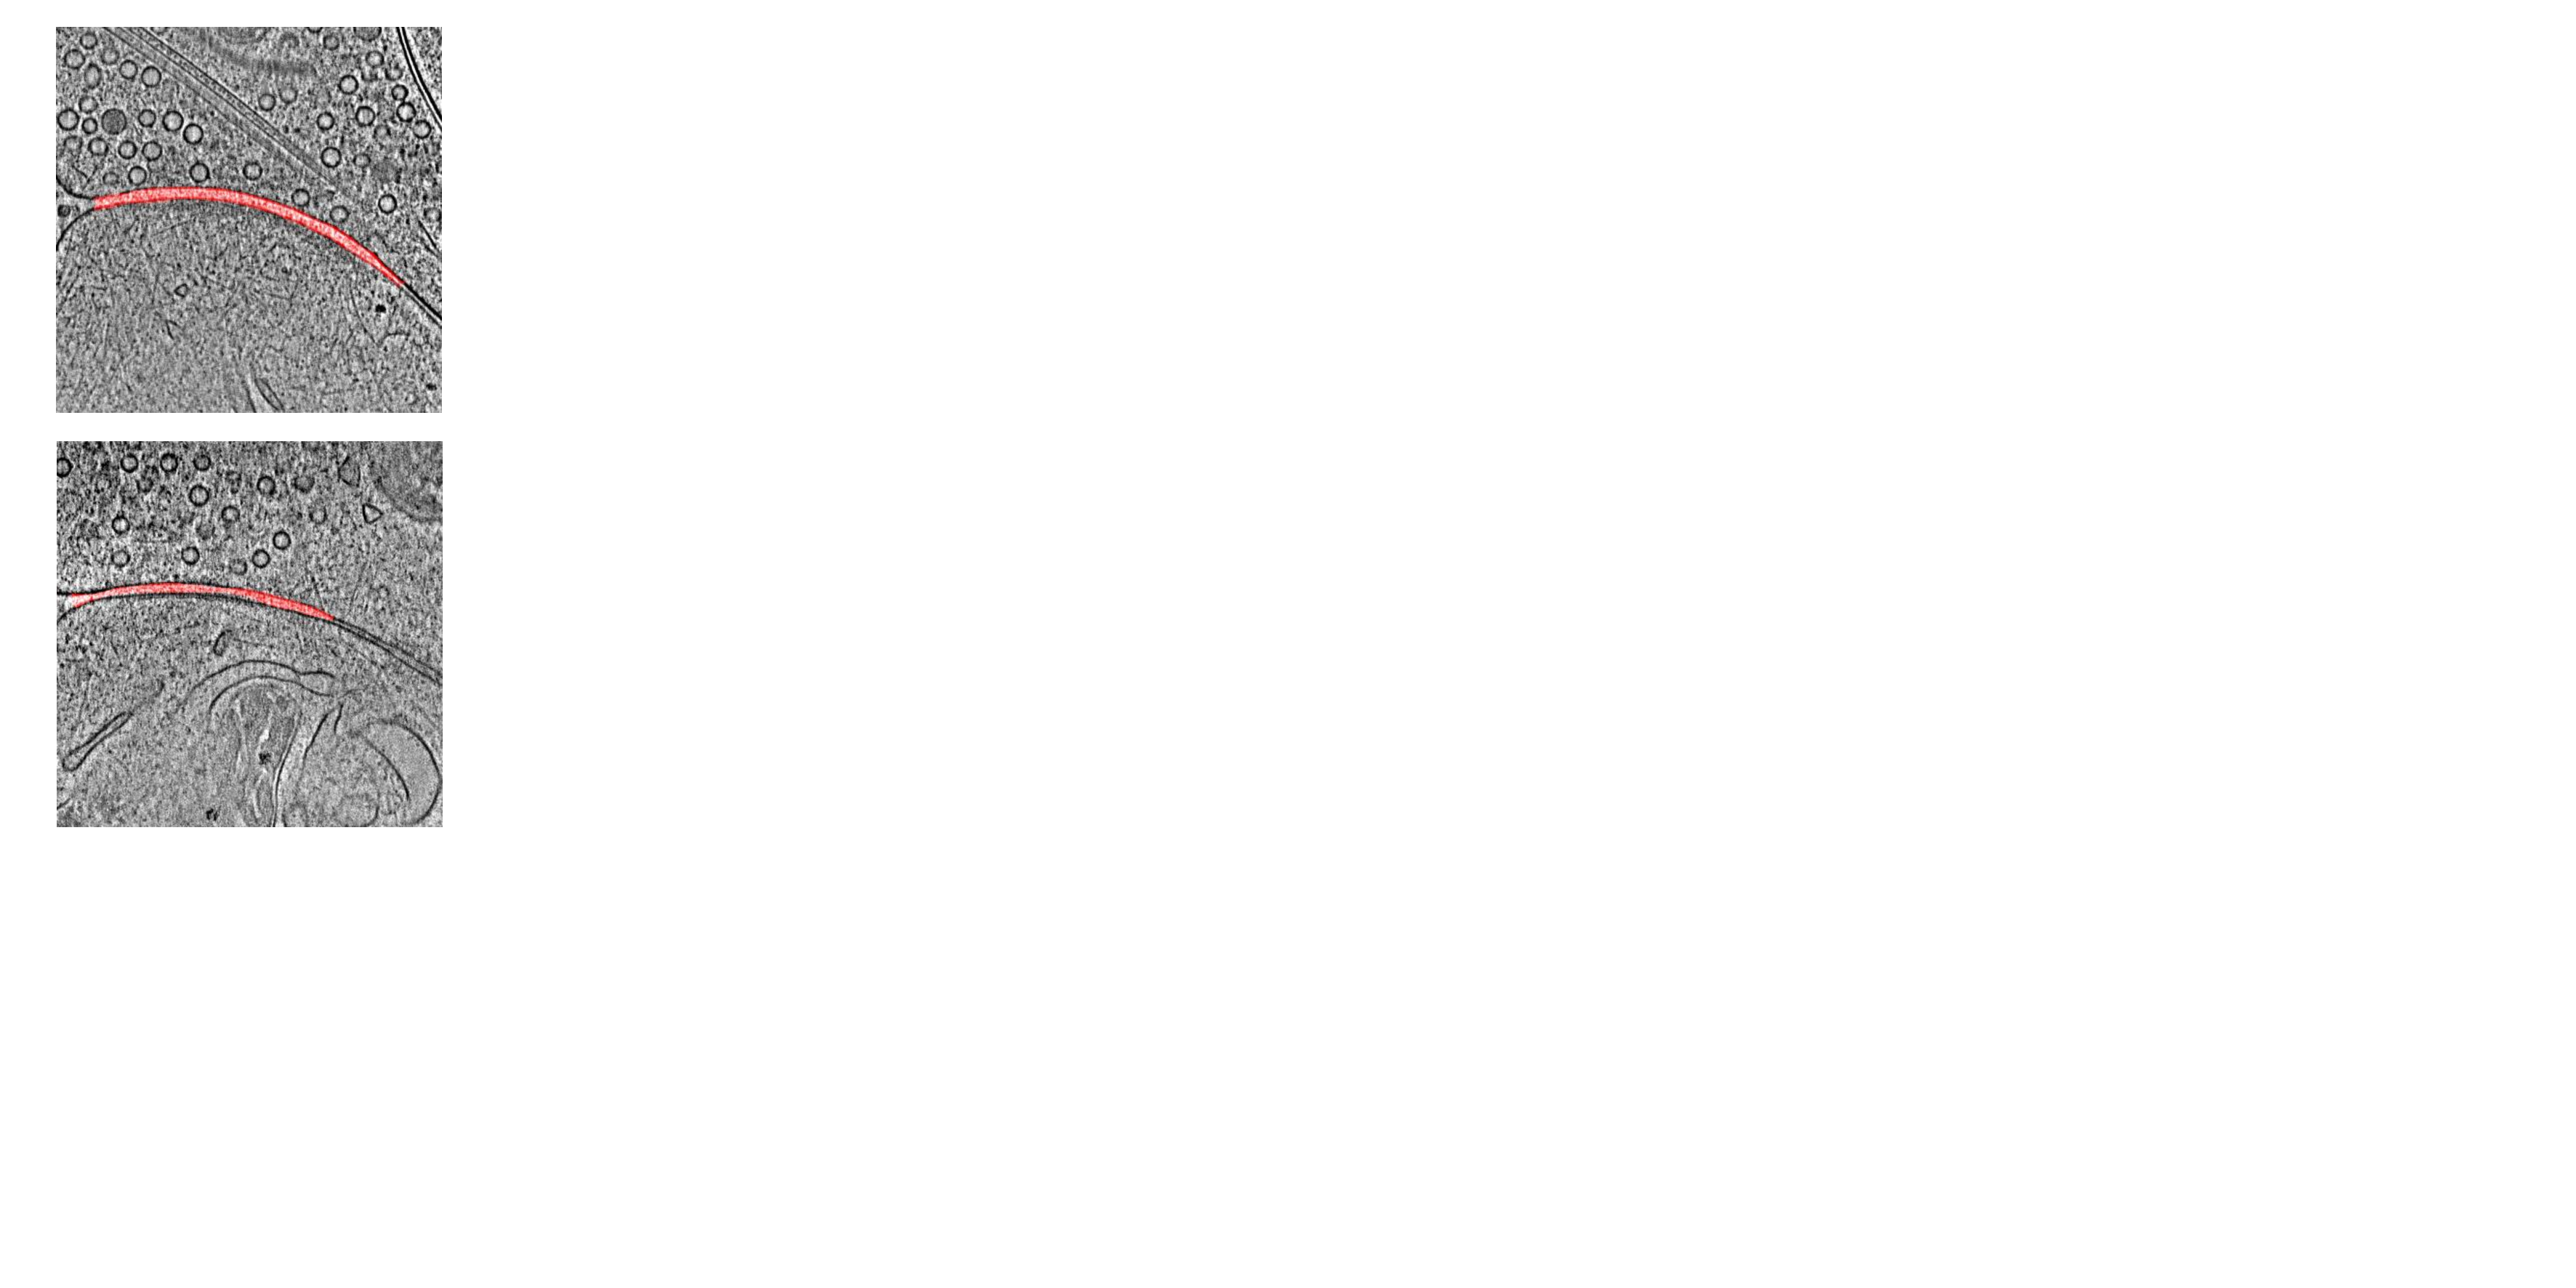
\includegraphics[height=2.3in,width=0.32\columnwidth]{figs/FigSeg1a.pdf}}
	%\hspace{0.2cm}
	\subfigure[FCN~\cite{Long2015}]{
		\label{fig:vesicle_DeepLab} %% label for second subfigure
		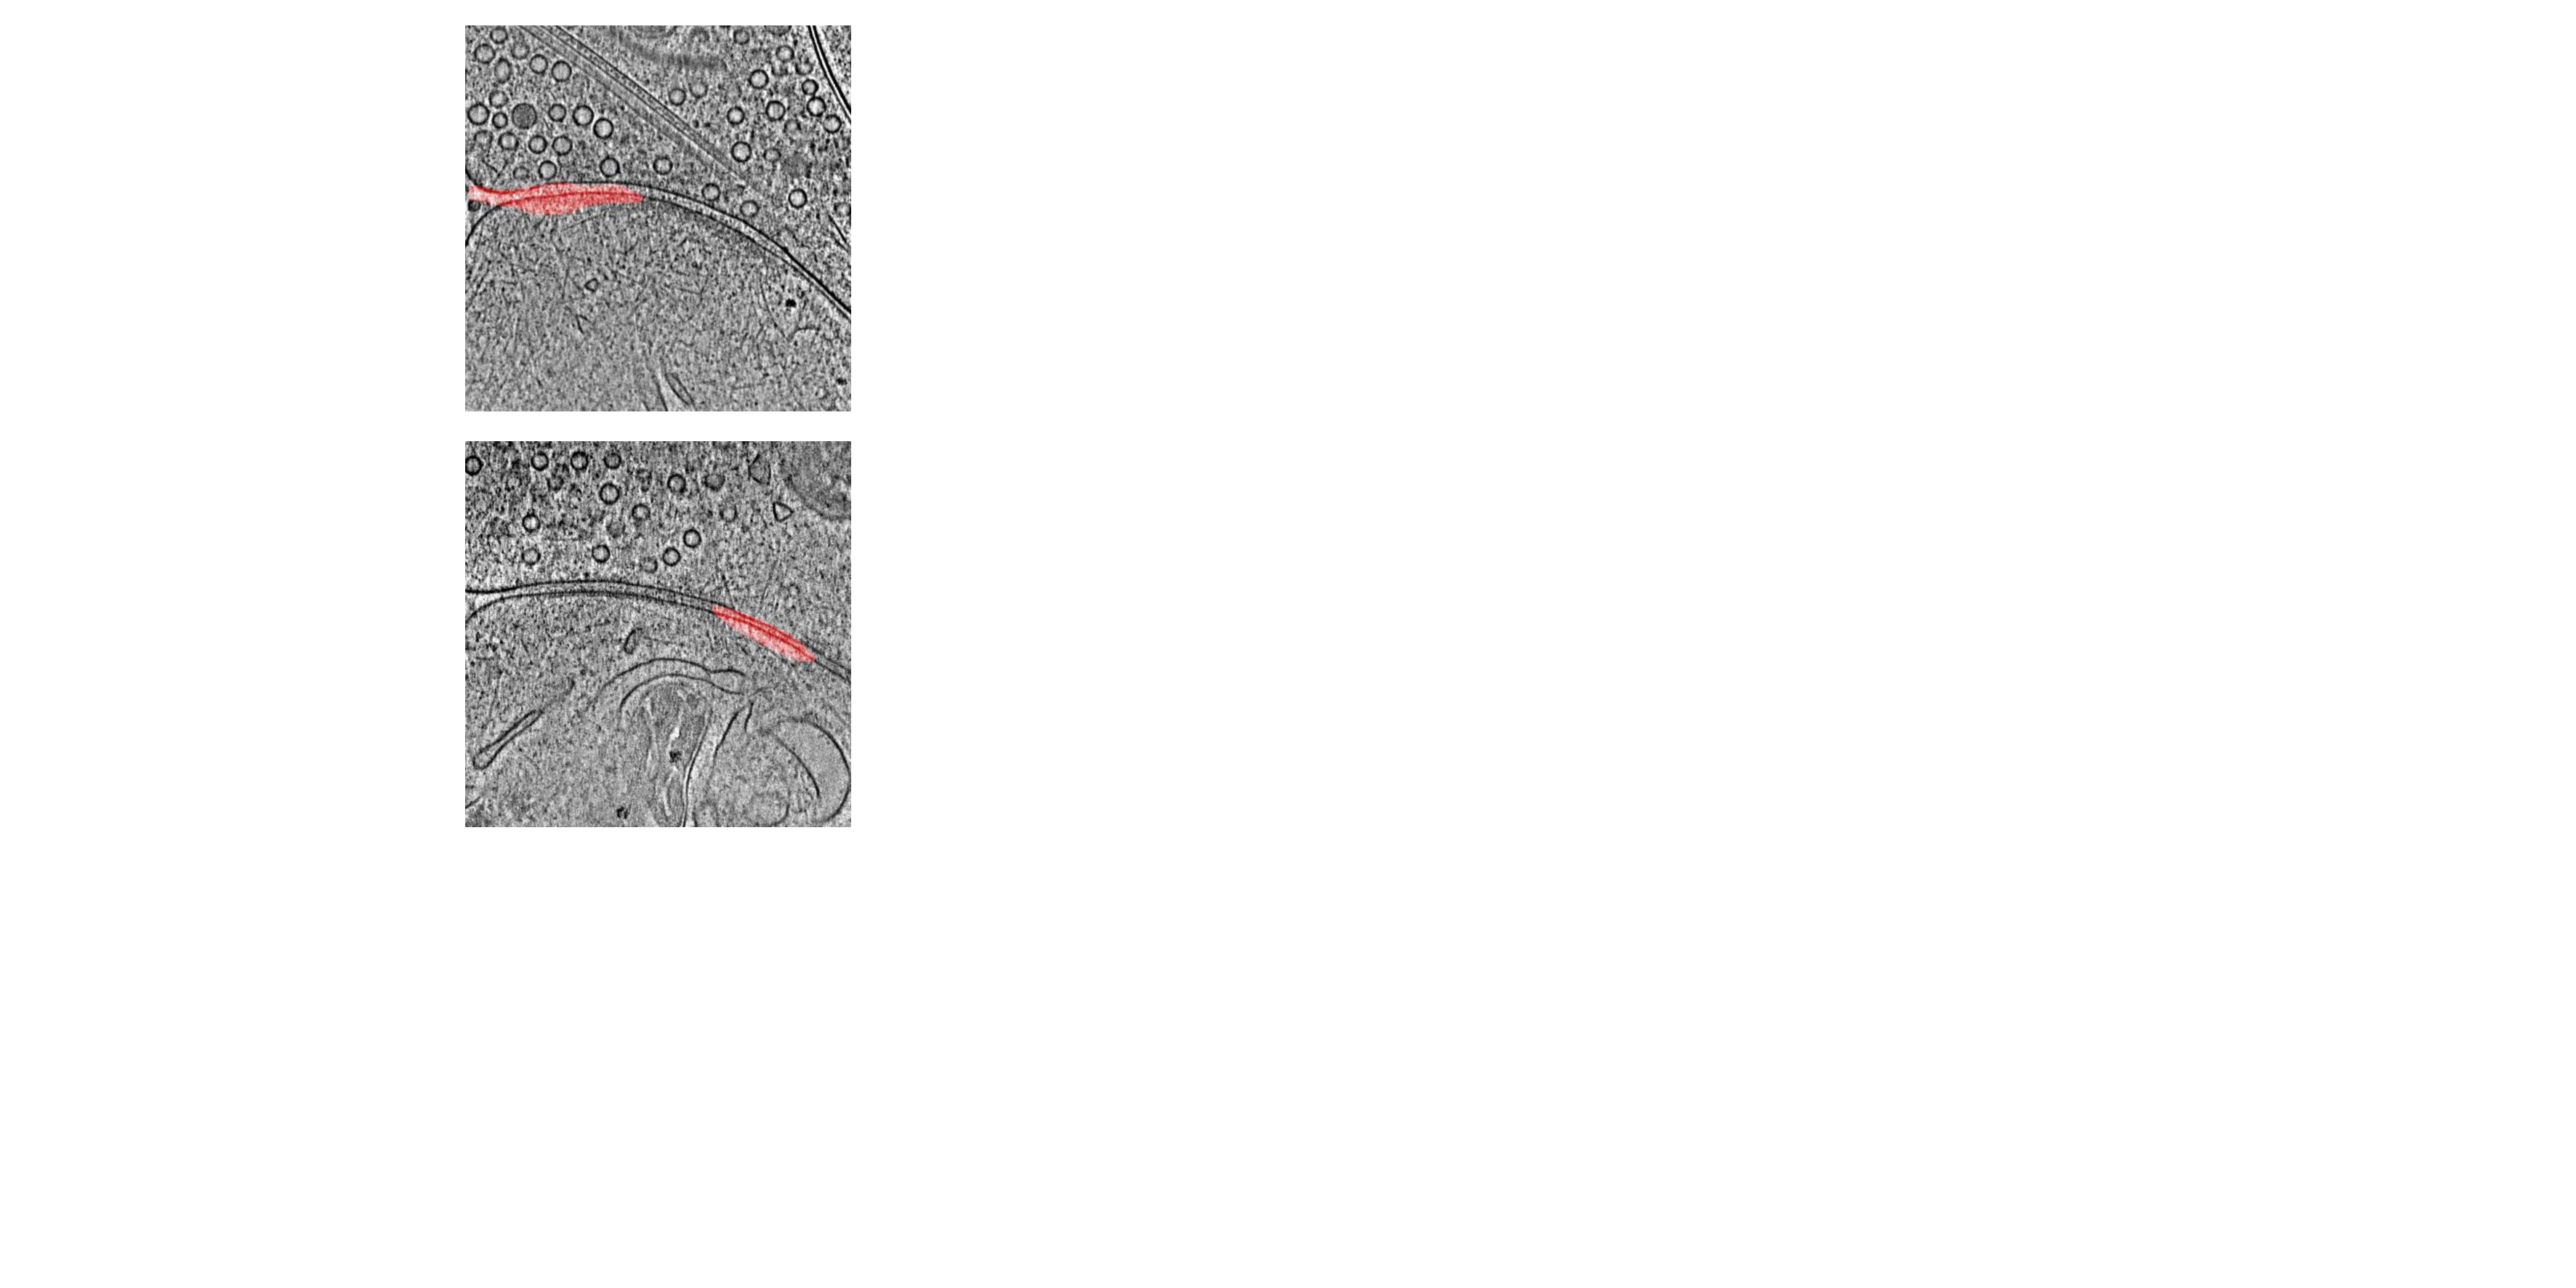
\includegraphics[height=2.3in,width=0.32\columnwidth]{figs/FigSeg1b.pdf}}
    %\hspace{0.2cm}
	\subfigure[U-net~\cite{Ronneberger2015}]{
		\label{fig:vesicle_Unet} %% label for second subfigure
		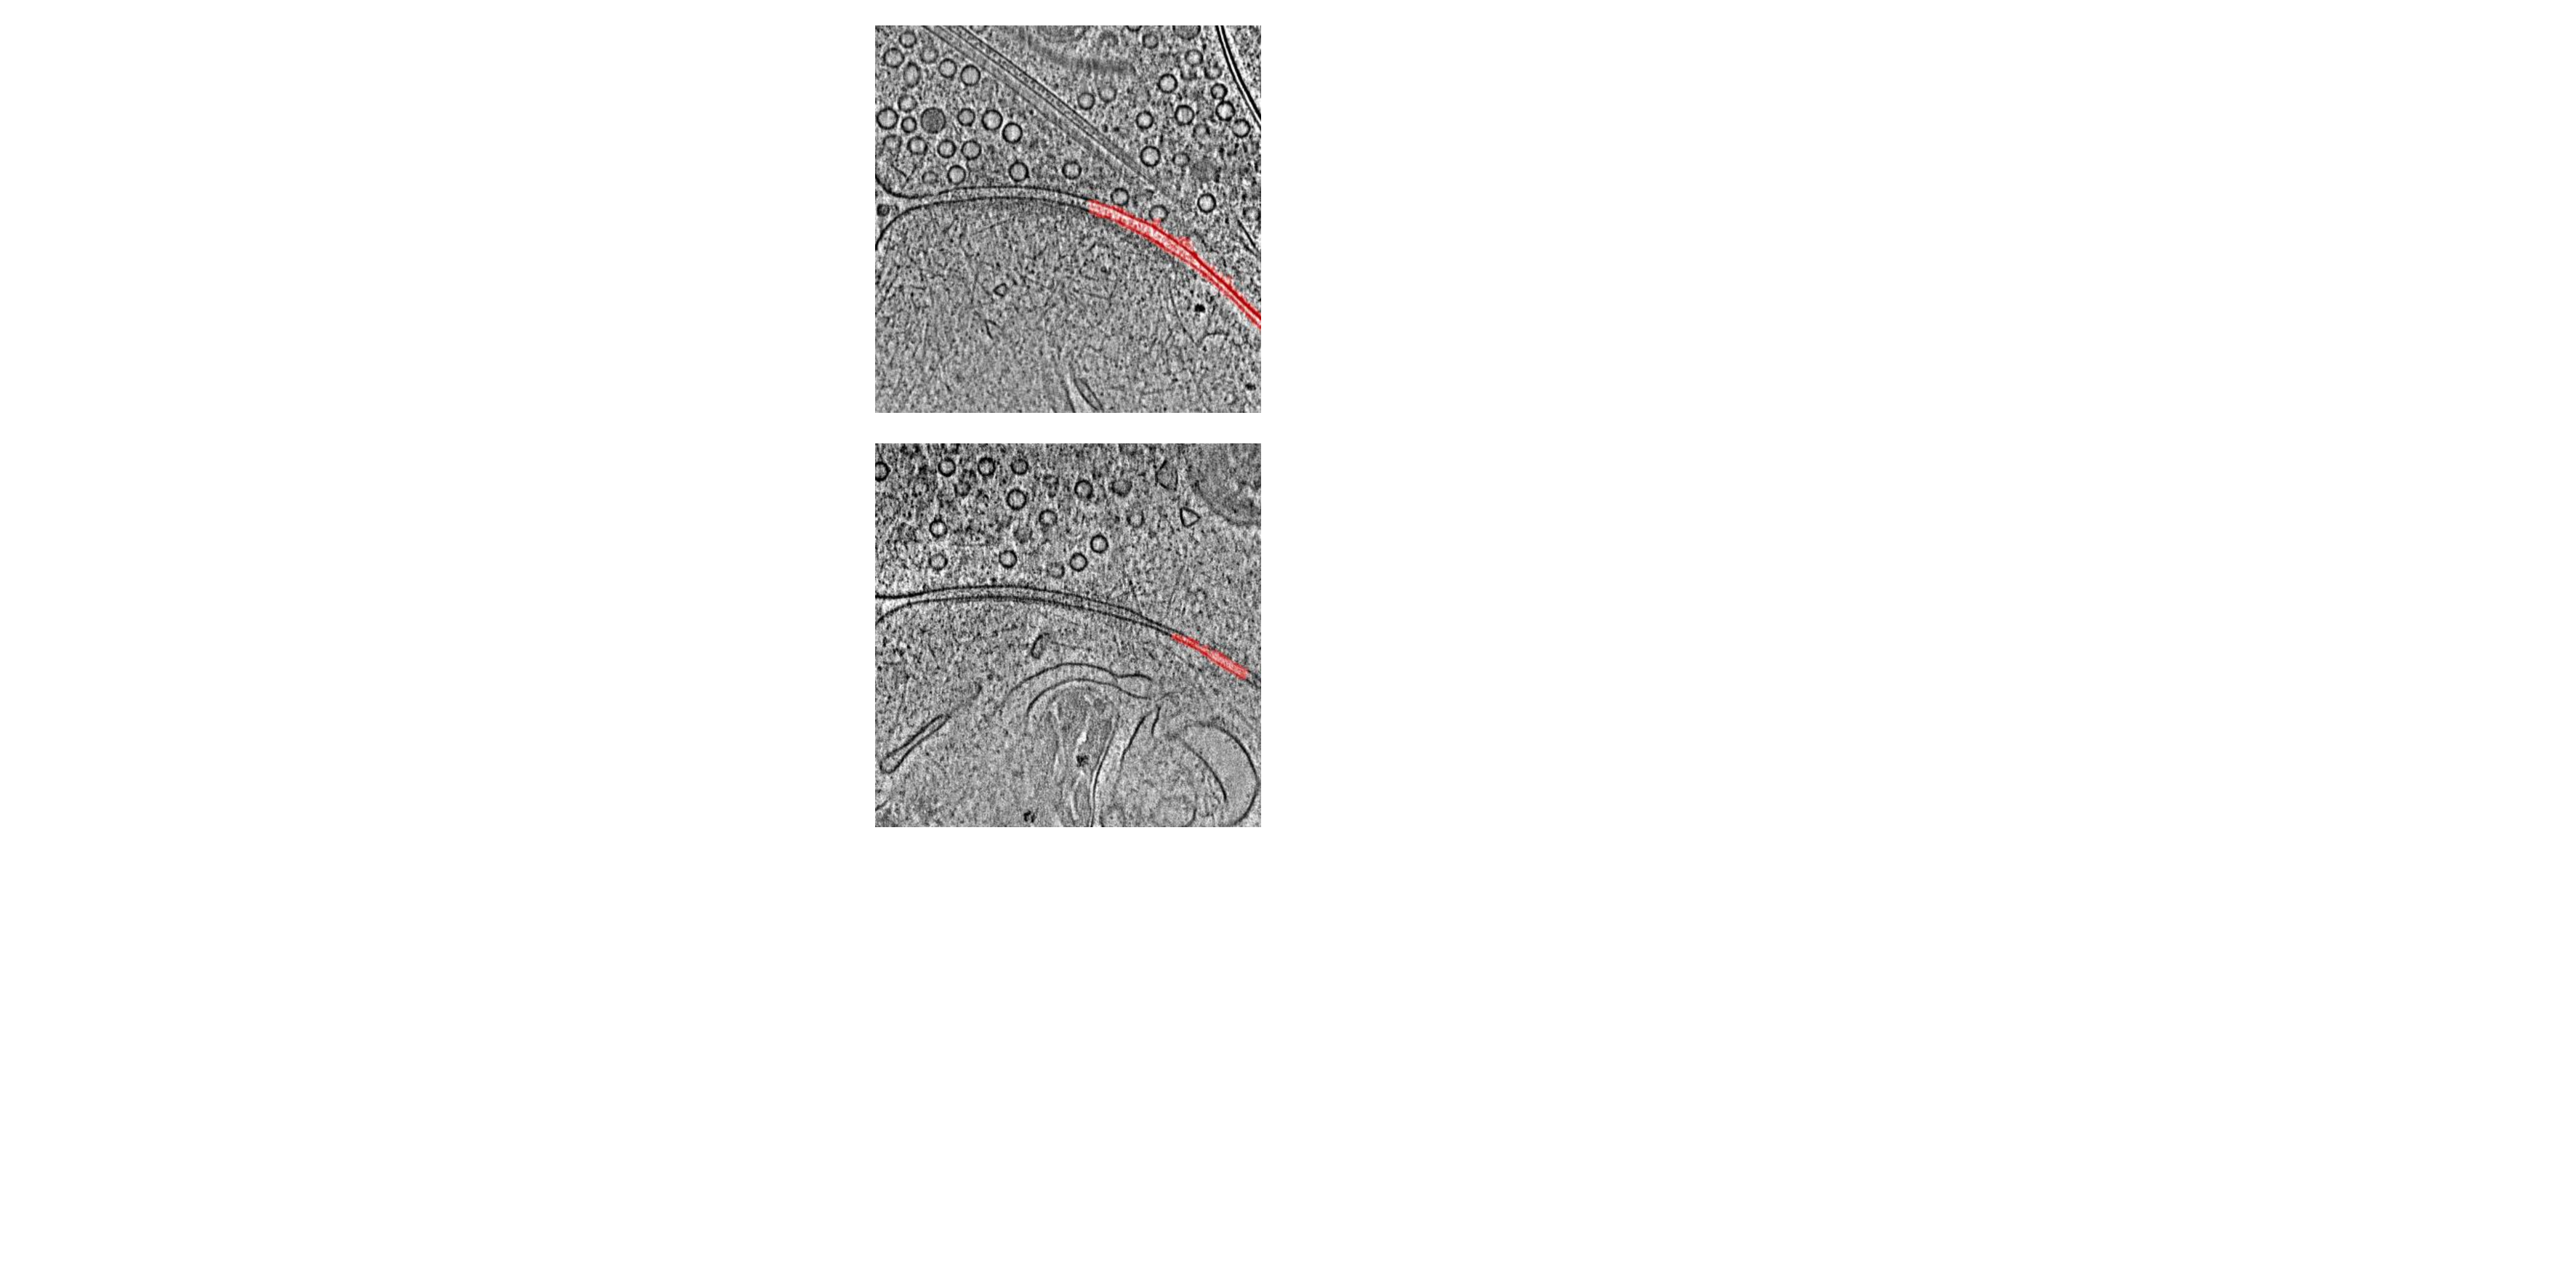
\includegraphics[height=2.3in,width=0.32\columnwidth]{figs/FigSeg1c.pdf}}
    %\hspace{0.2cm}
	\subfigure[DeepLab~\cite{Chen2016a}]{
		\label{fig:vesicle_dcan} %% label for second subfigure
		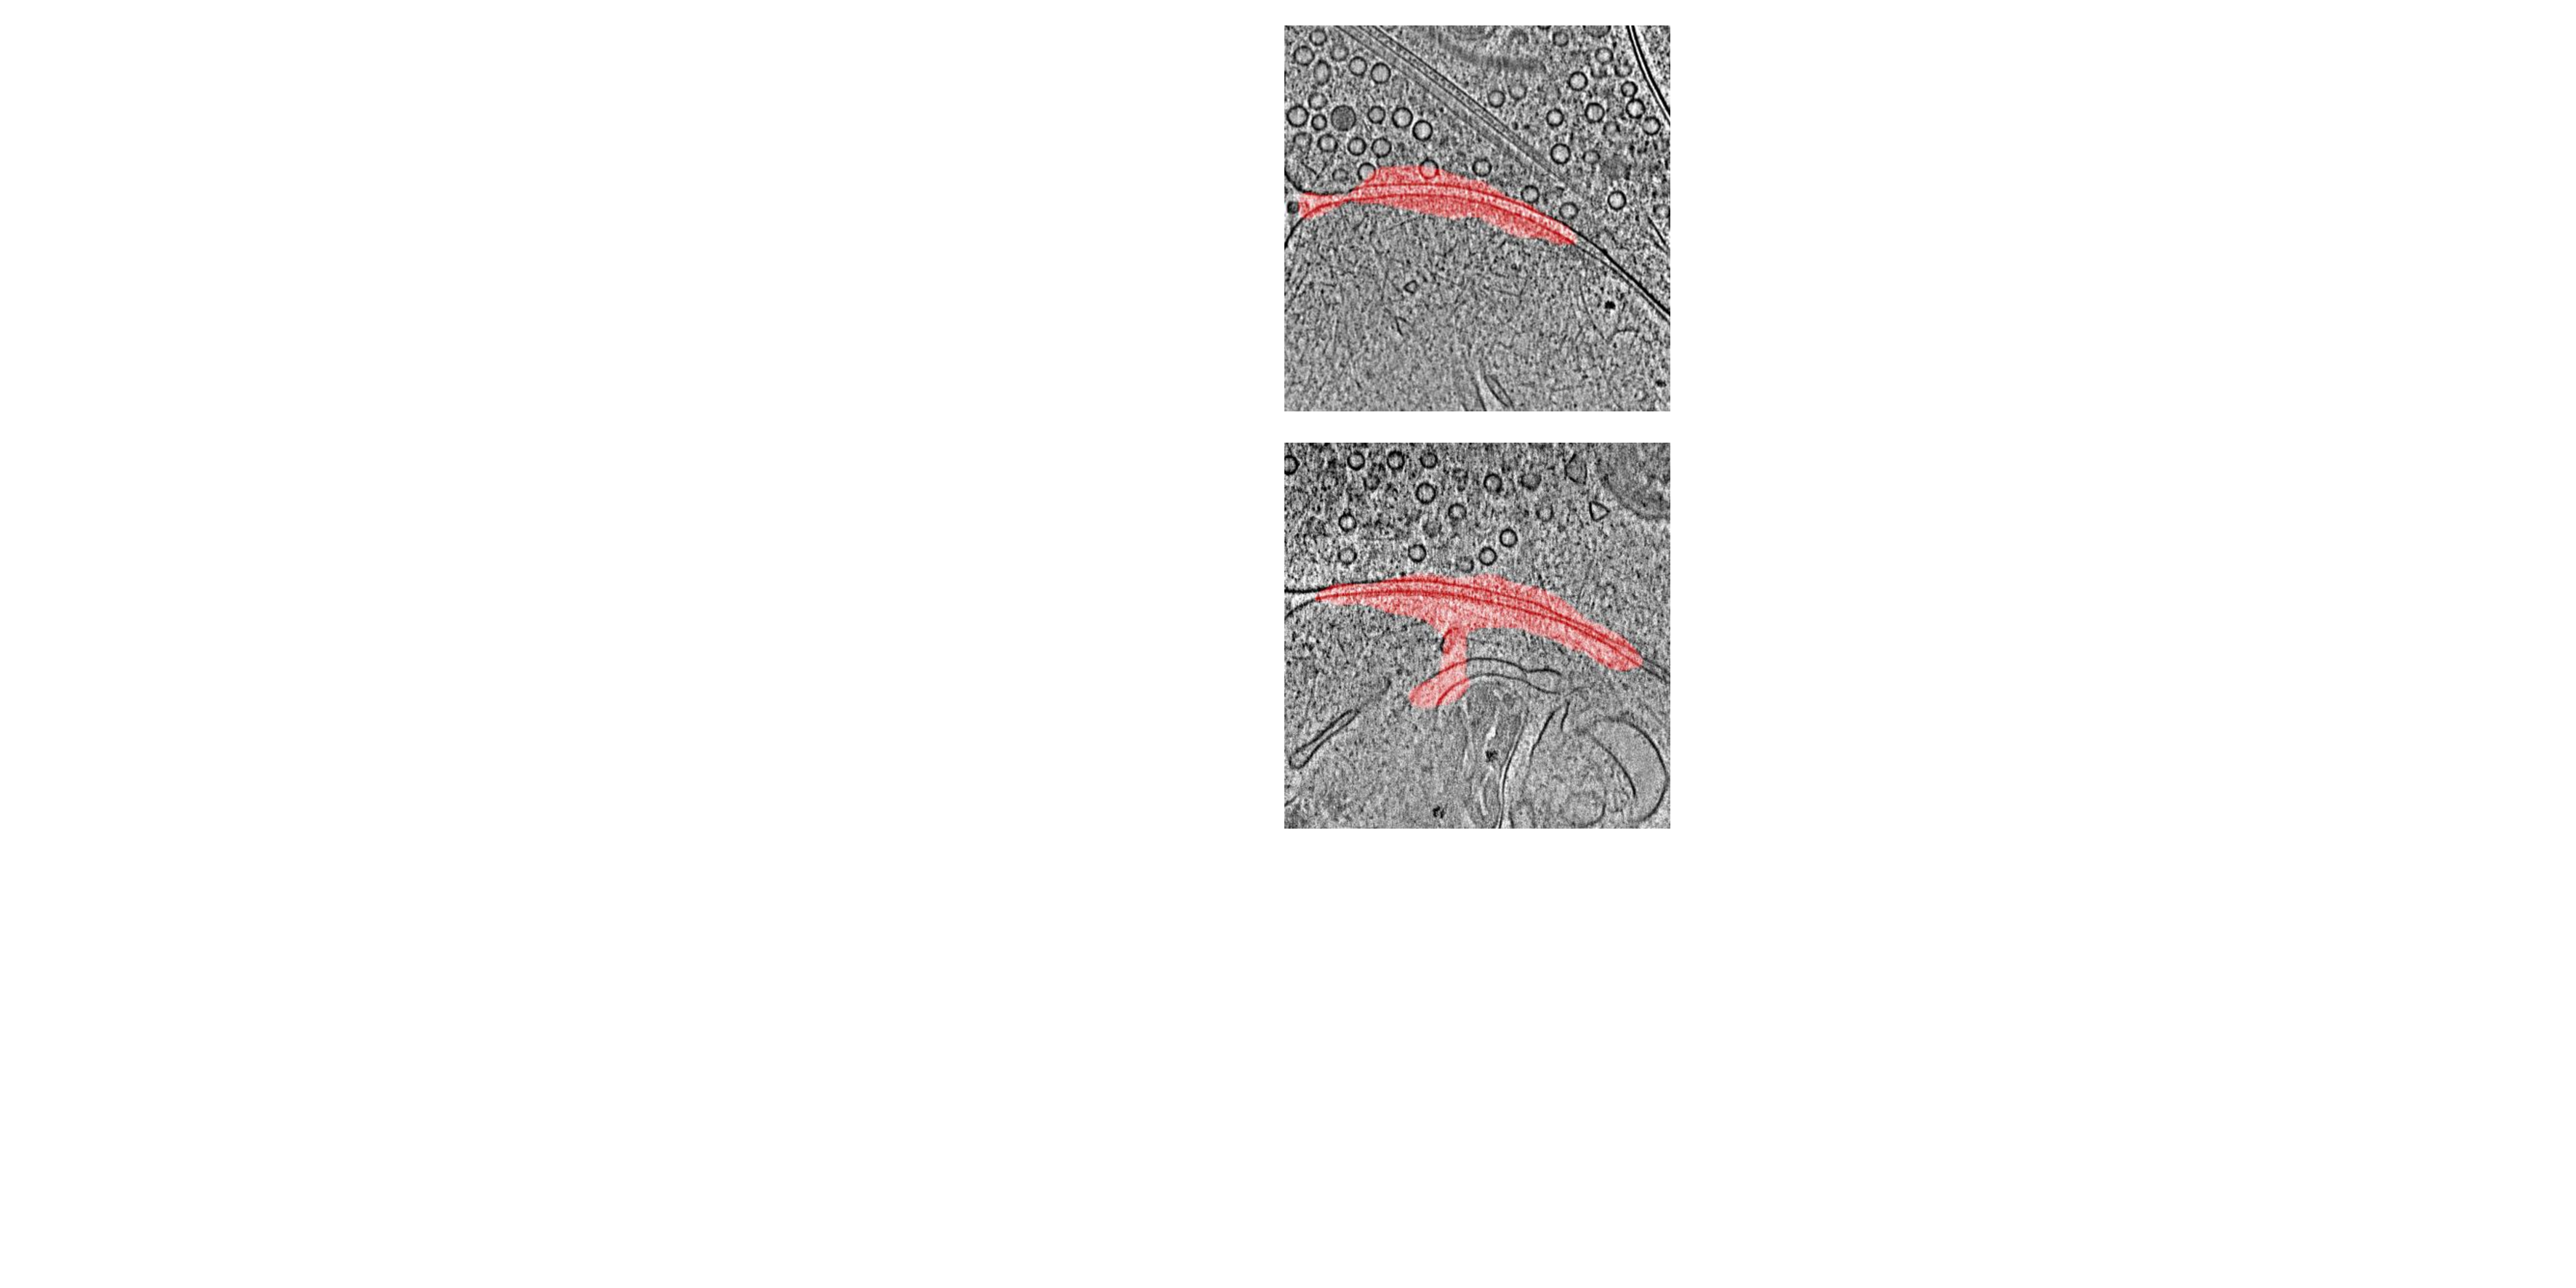
\includegraphics[height=2.3in,width=0.32\columnwidth]{figs/FigSeg1d.pdf}}
    %\hspace{0.2cm}
	\subfigure[PSPNet~\cite{Zhao2016}]{
		\label{fig:vesicle_dsan} %% label for second subfigure
		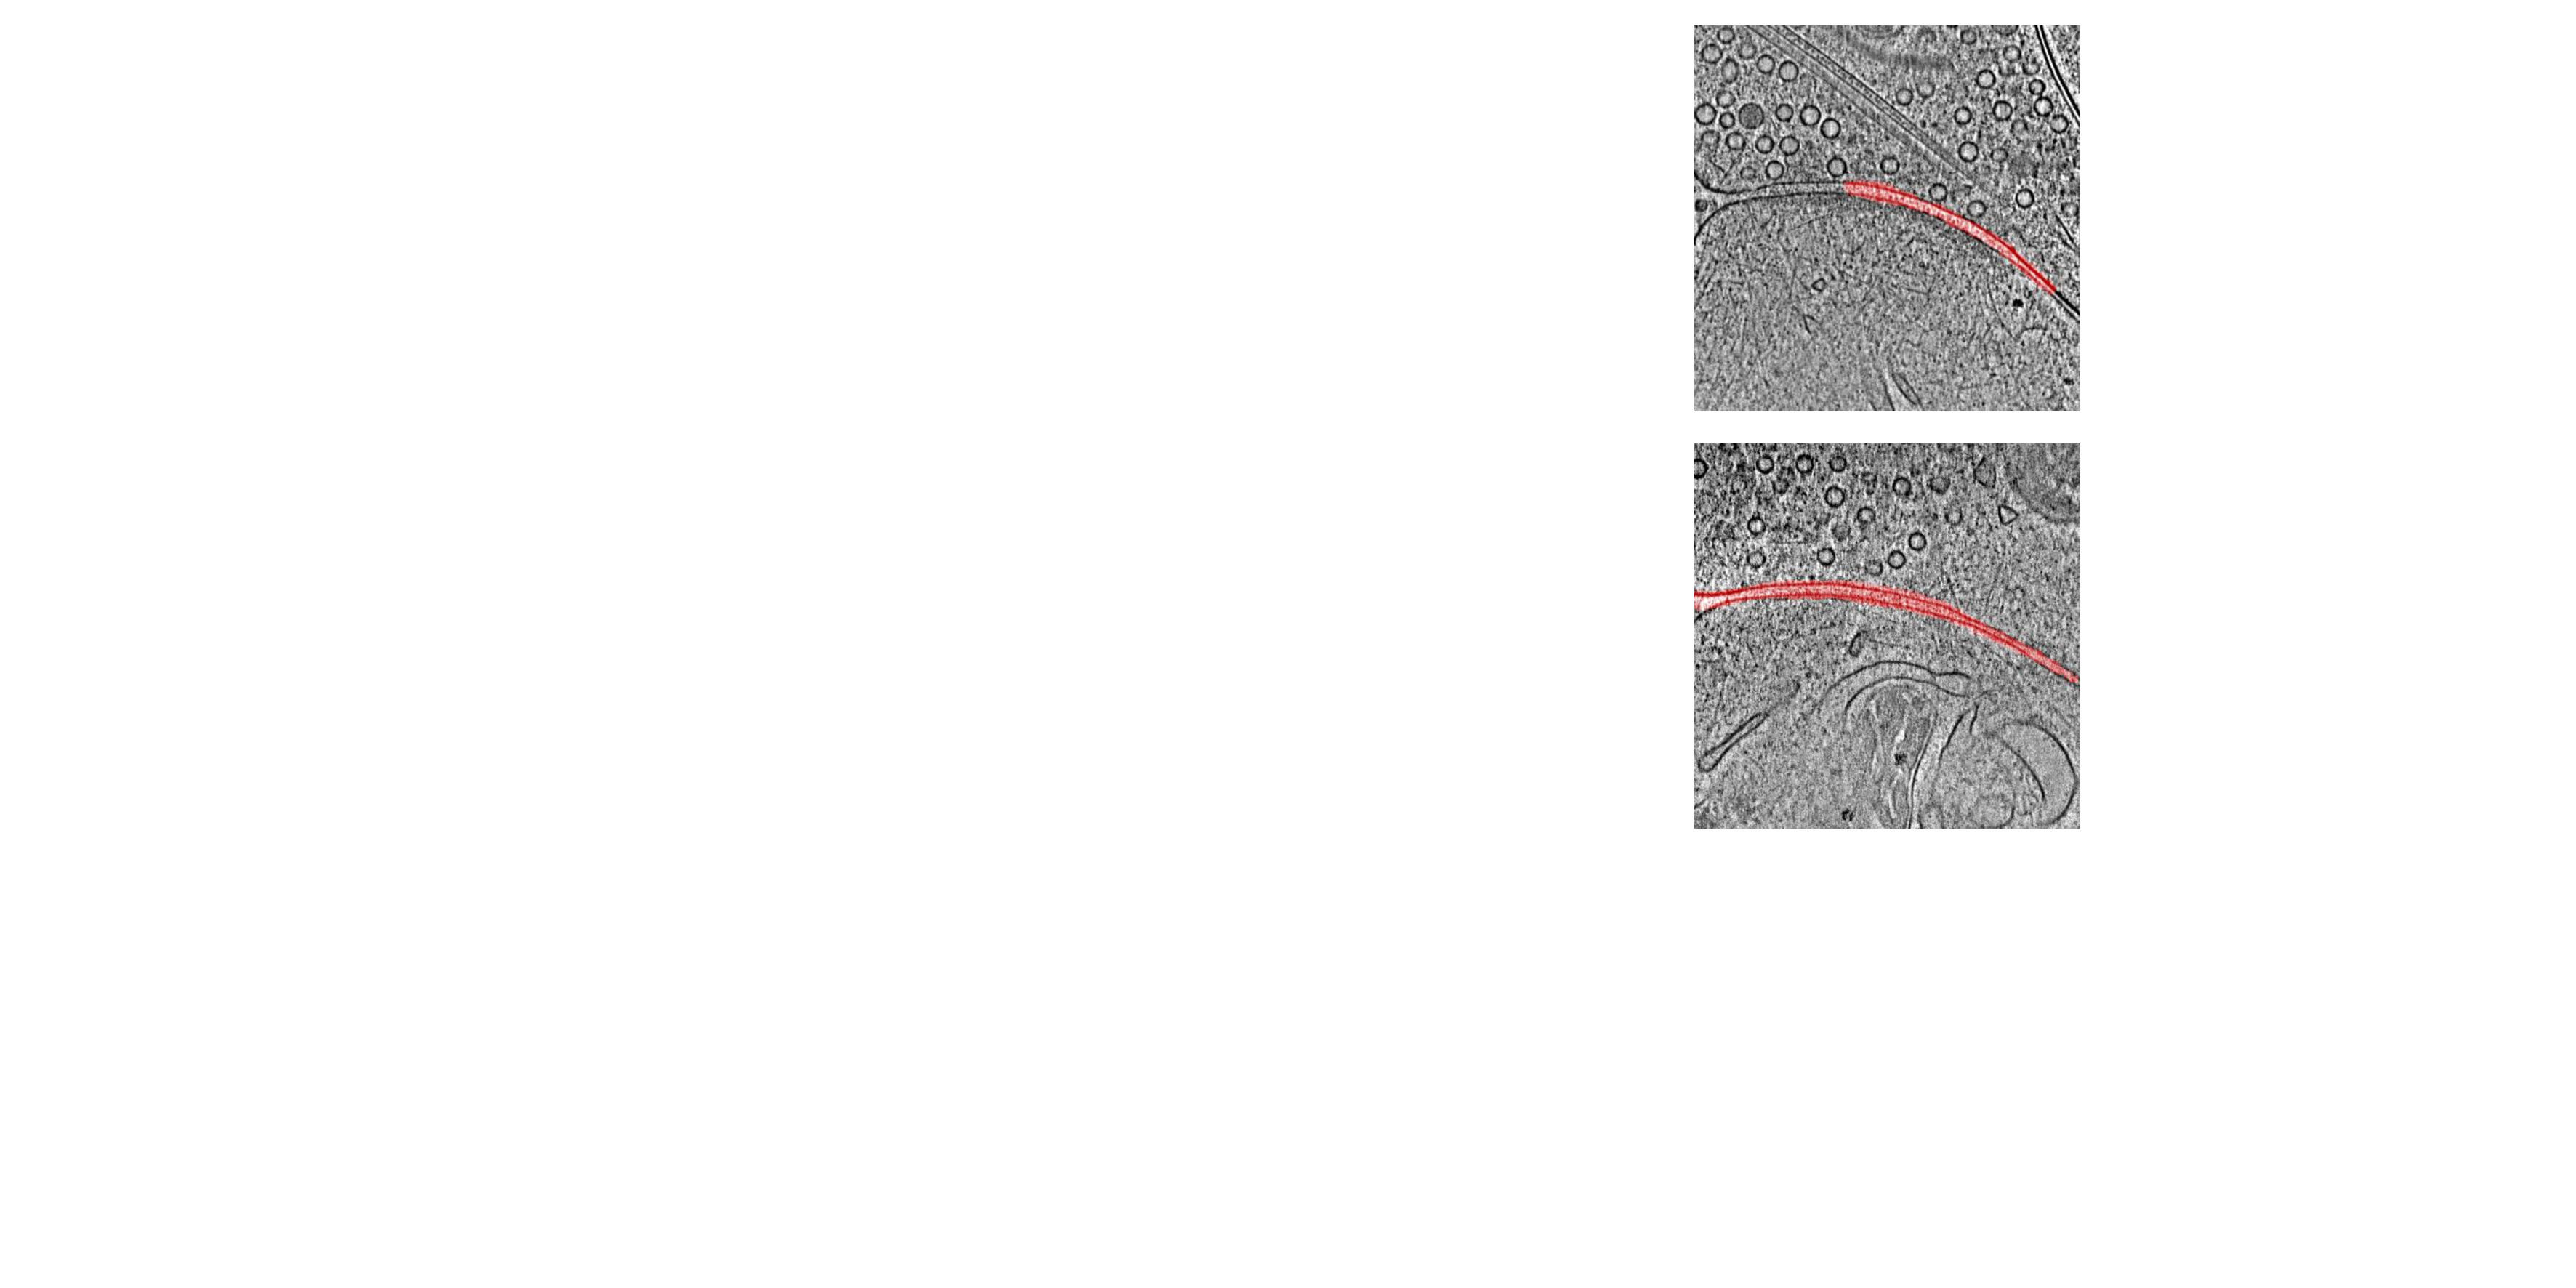
\includegraphics[height=2.3in,width=0.32\columnwidth]{figs/FigSeg1e.pdf}}
    %\hspace{0.2cm}
	\subfigure[Ours]{
		\label{fig:vesicle_gt} %% label for second subfigure
		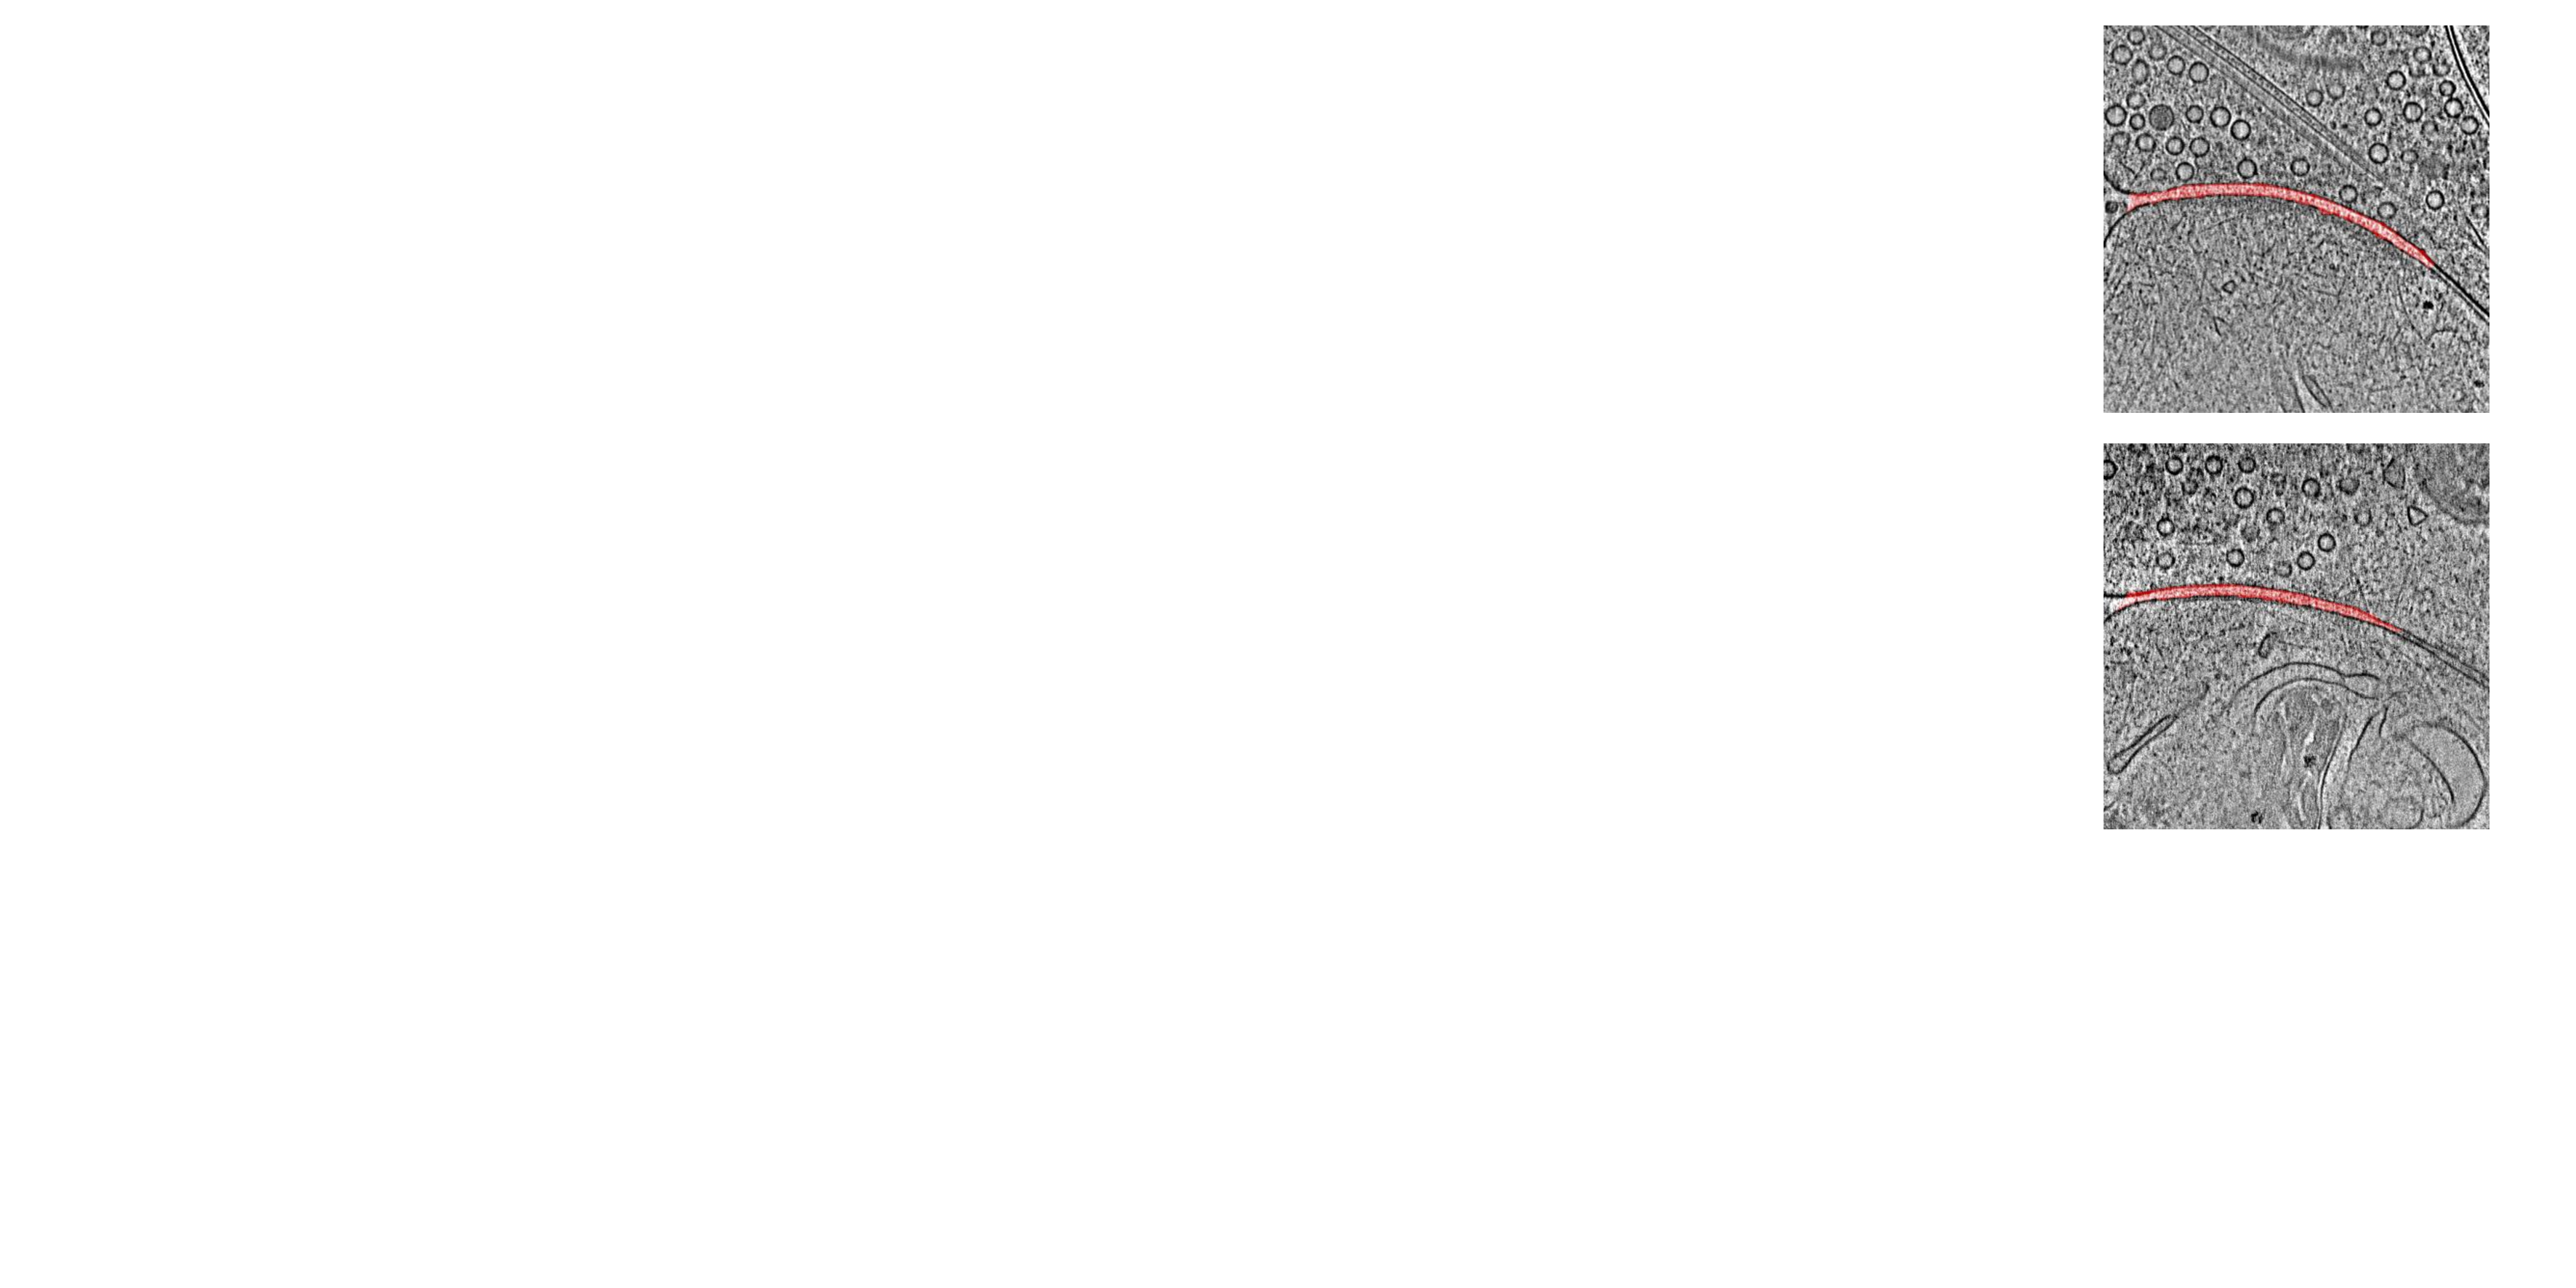
\includegraphics[height=2.3in,width=0.32\columnwidth]{figs/FigSeg1f.pdf}}

	\caption{ Results produced by state of the art segmentations methods and our model.  }
	\label{FigSeg1}
\end{figure*}


\begin{figure}
	\centering
	\subfigure[FCN~\cite{Long2015}]{
		\label{fig:seg2:fcn} %% label for first subfigure
		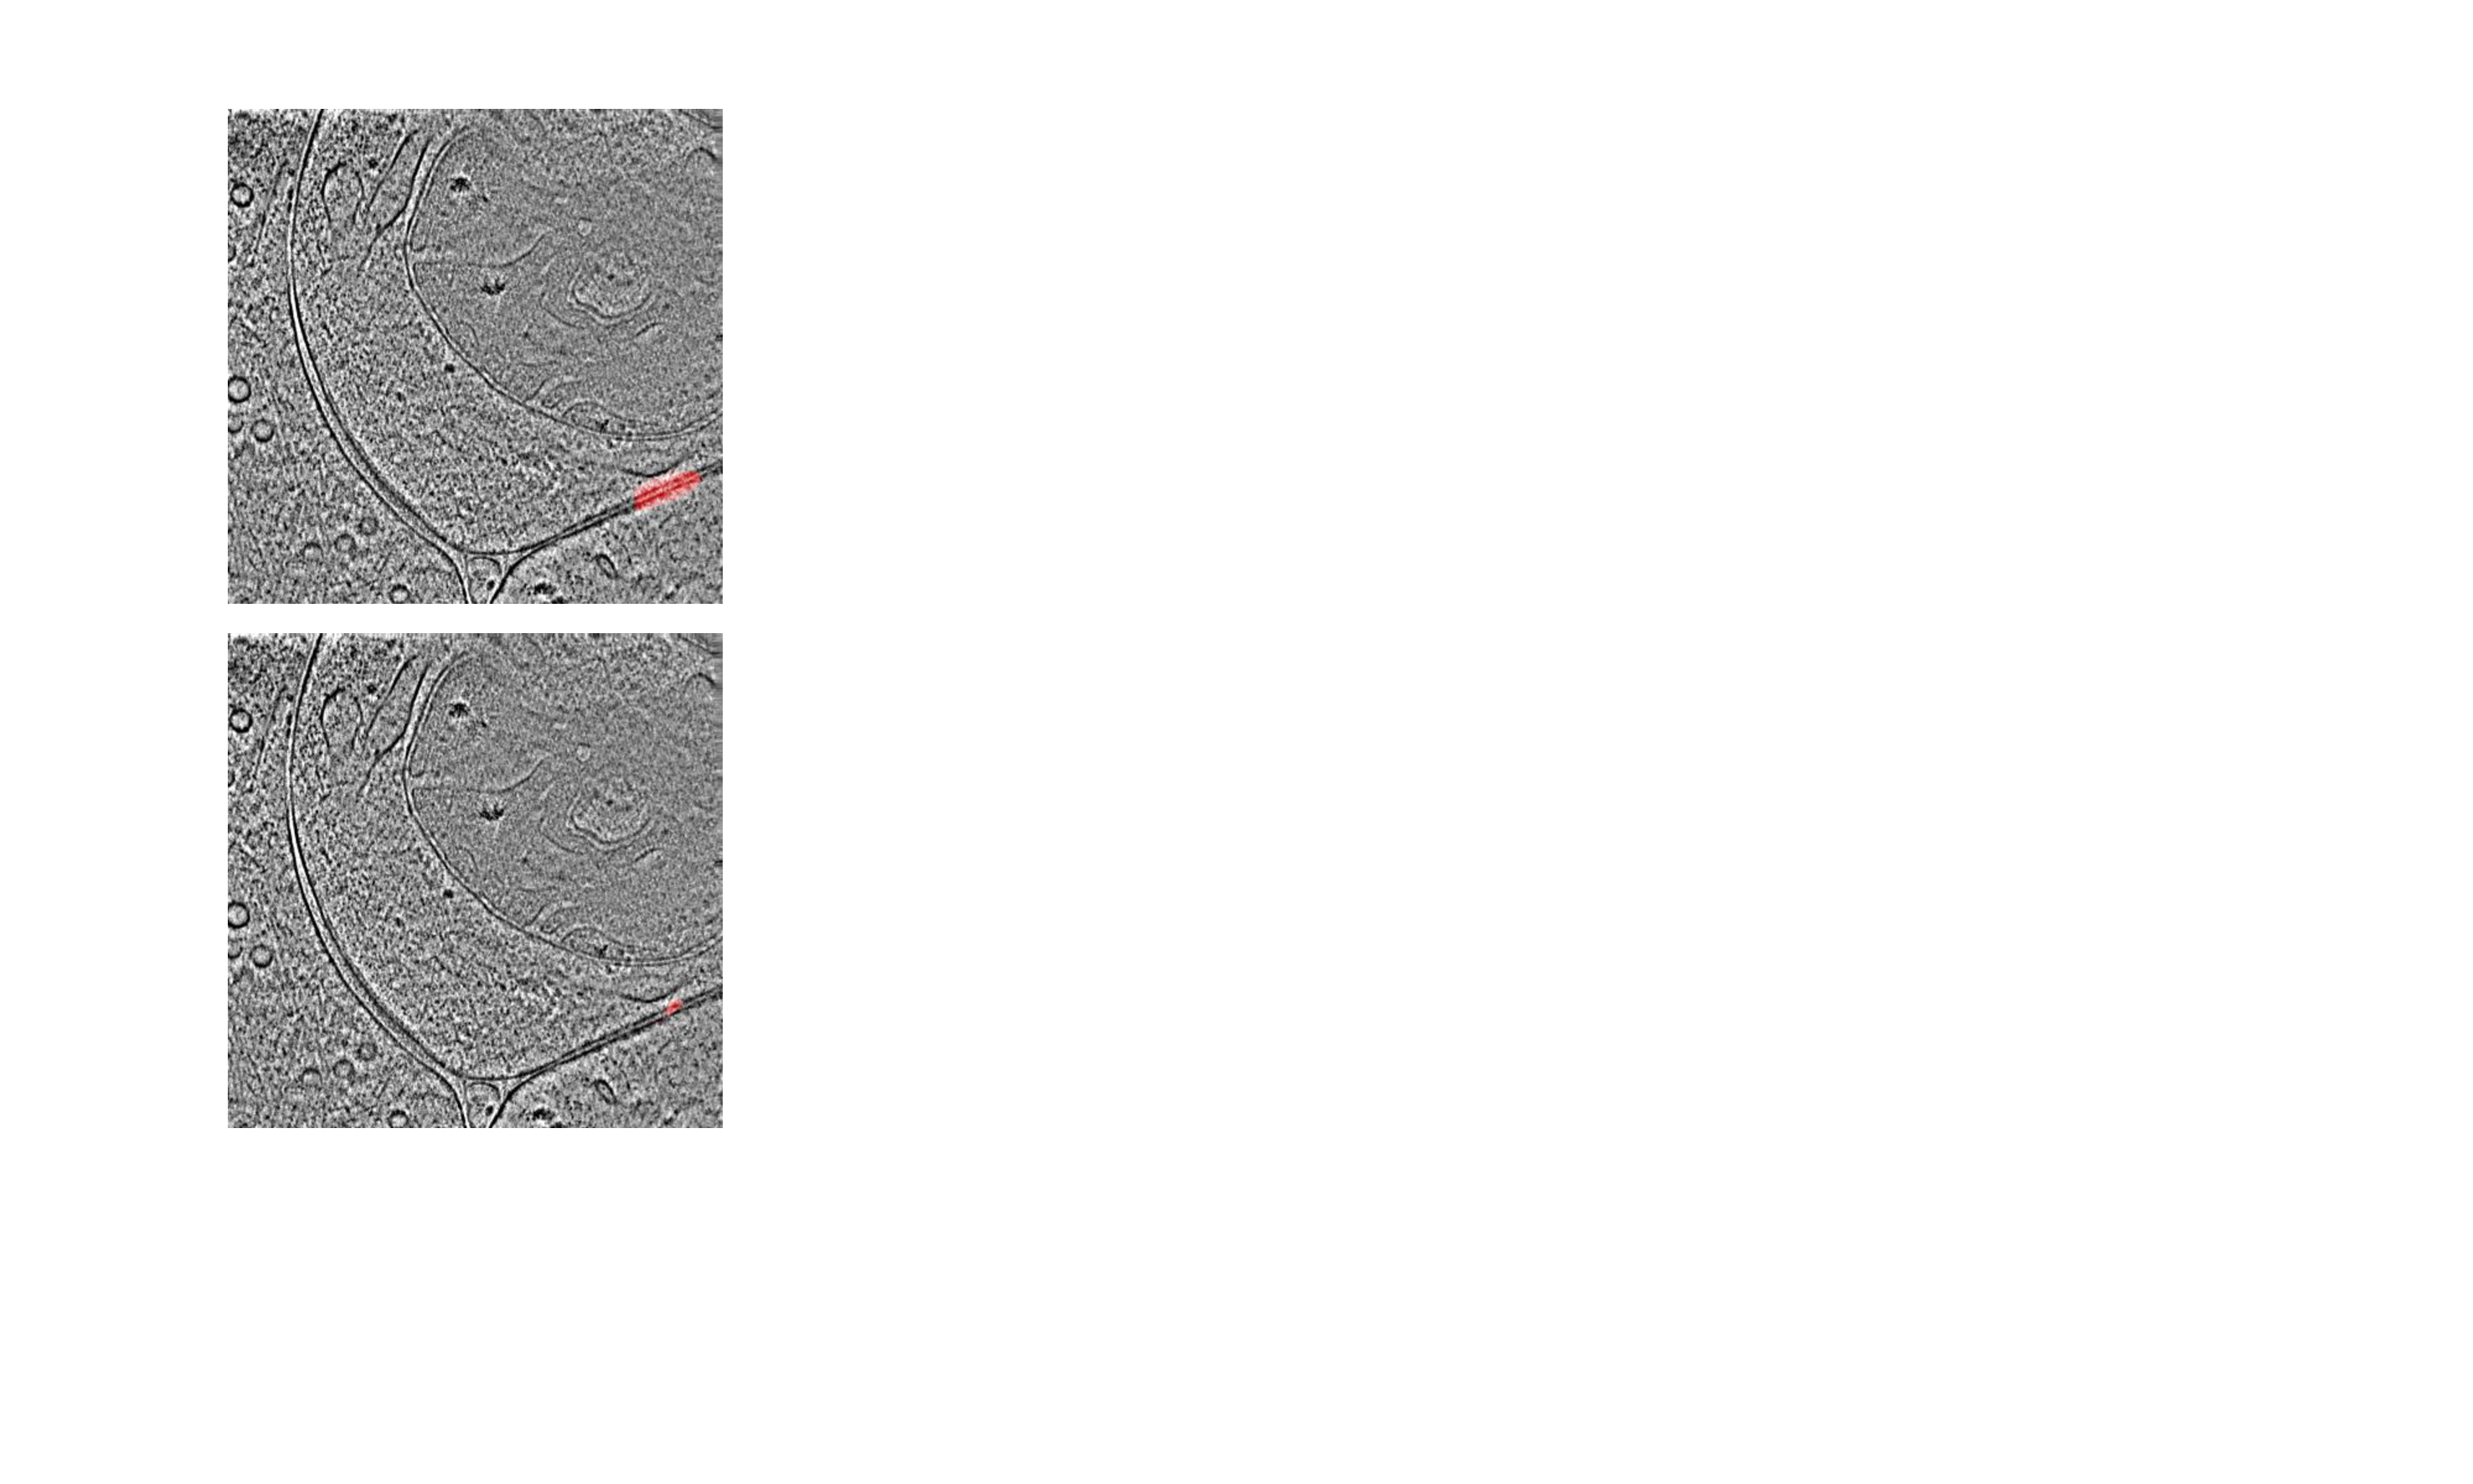
\includegraphics[height=1.6in,width=0.23\columnwidth]{figs/FigSeg2a.pdf}}
	%\hspace{0.01cm}
	\subfigure[U-net~\cite{Ronneberger2015}]{
		\label{fig:seg2:unet} %% label for second subfigure
		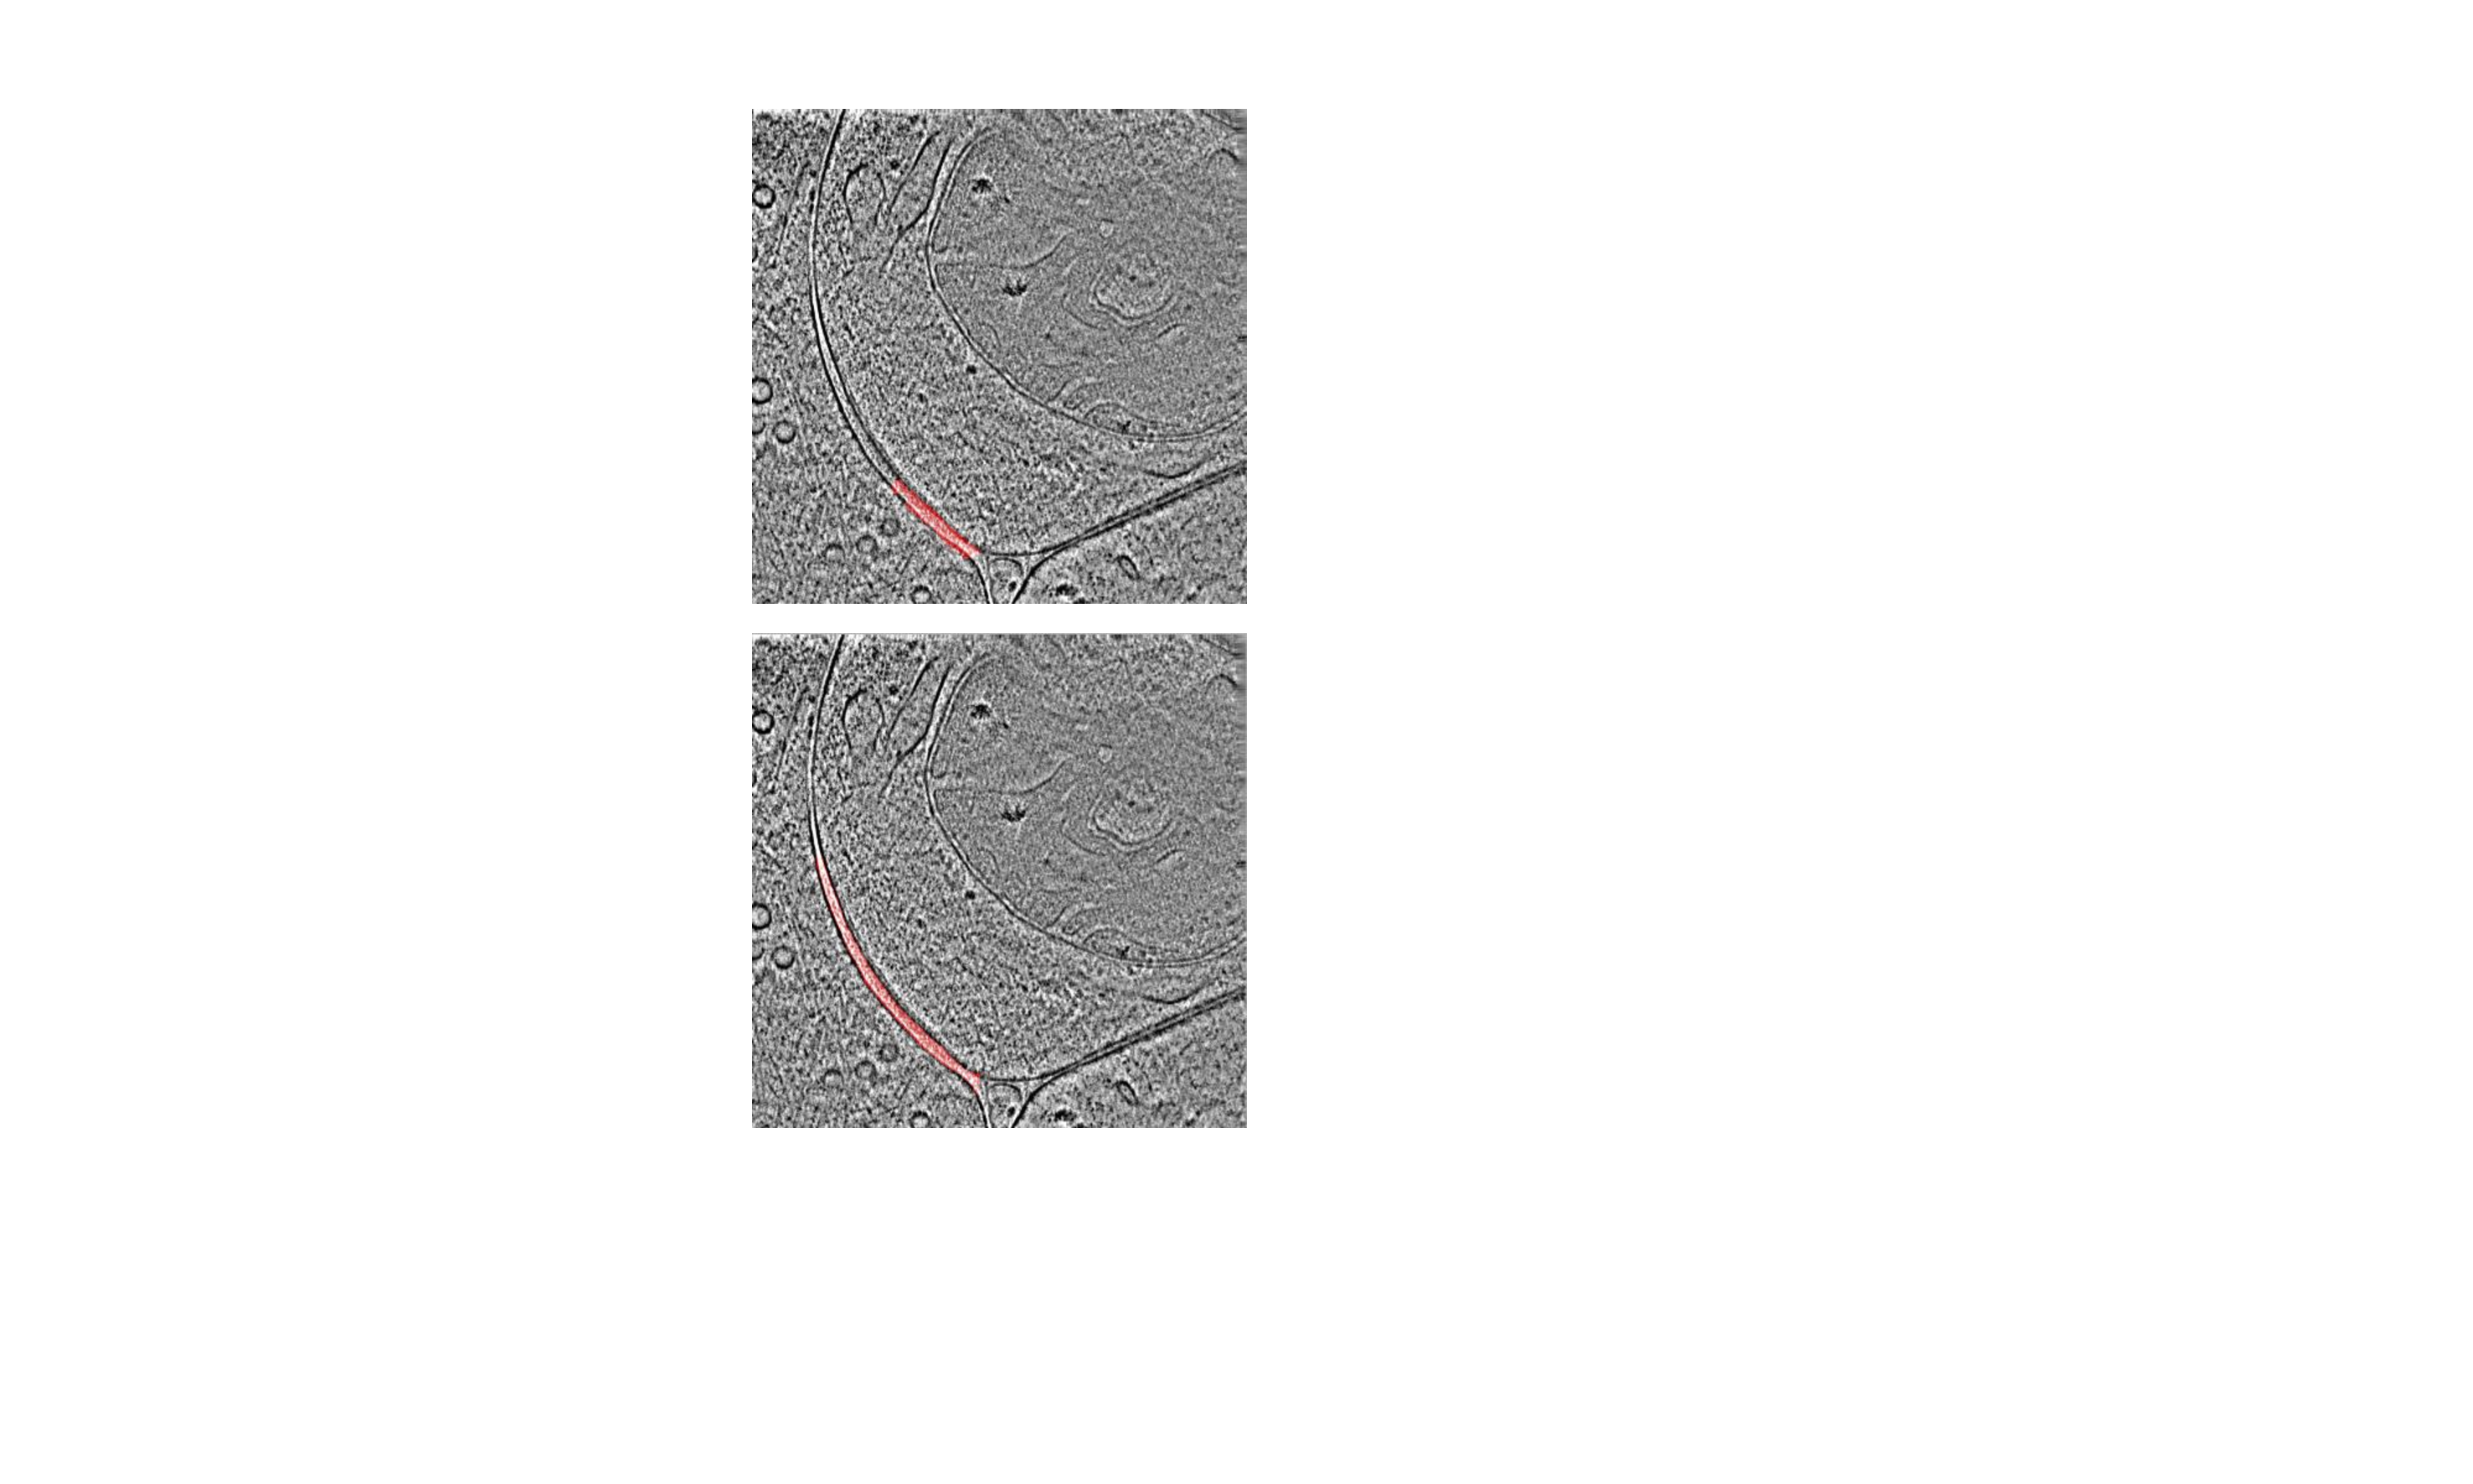
\includegraphics[height=1.6in,width=0.23\columnwidth]{figs/FigSeg2b.pdf}}
    %\hspace{0.05cm}
	\subfigure[DeepLab~\cite{Chen2016a}]{
		\label{fig:seg2:deeplab} %% label for second subfigure
		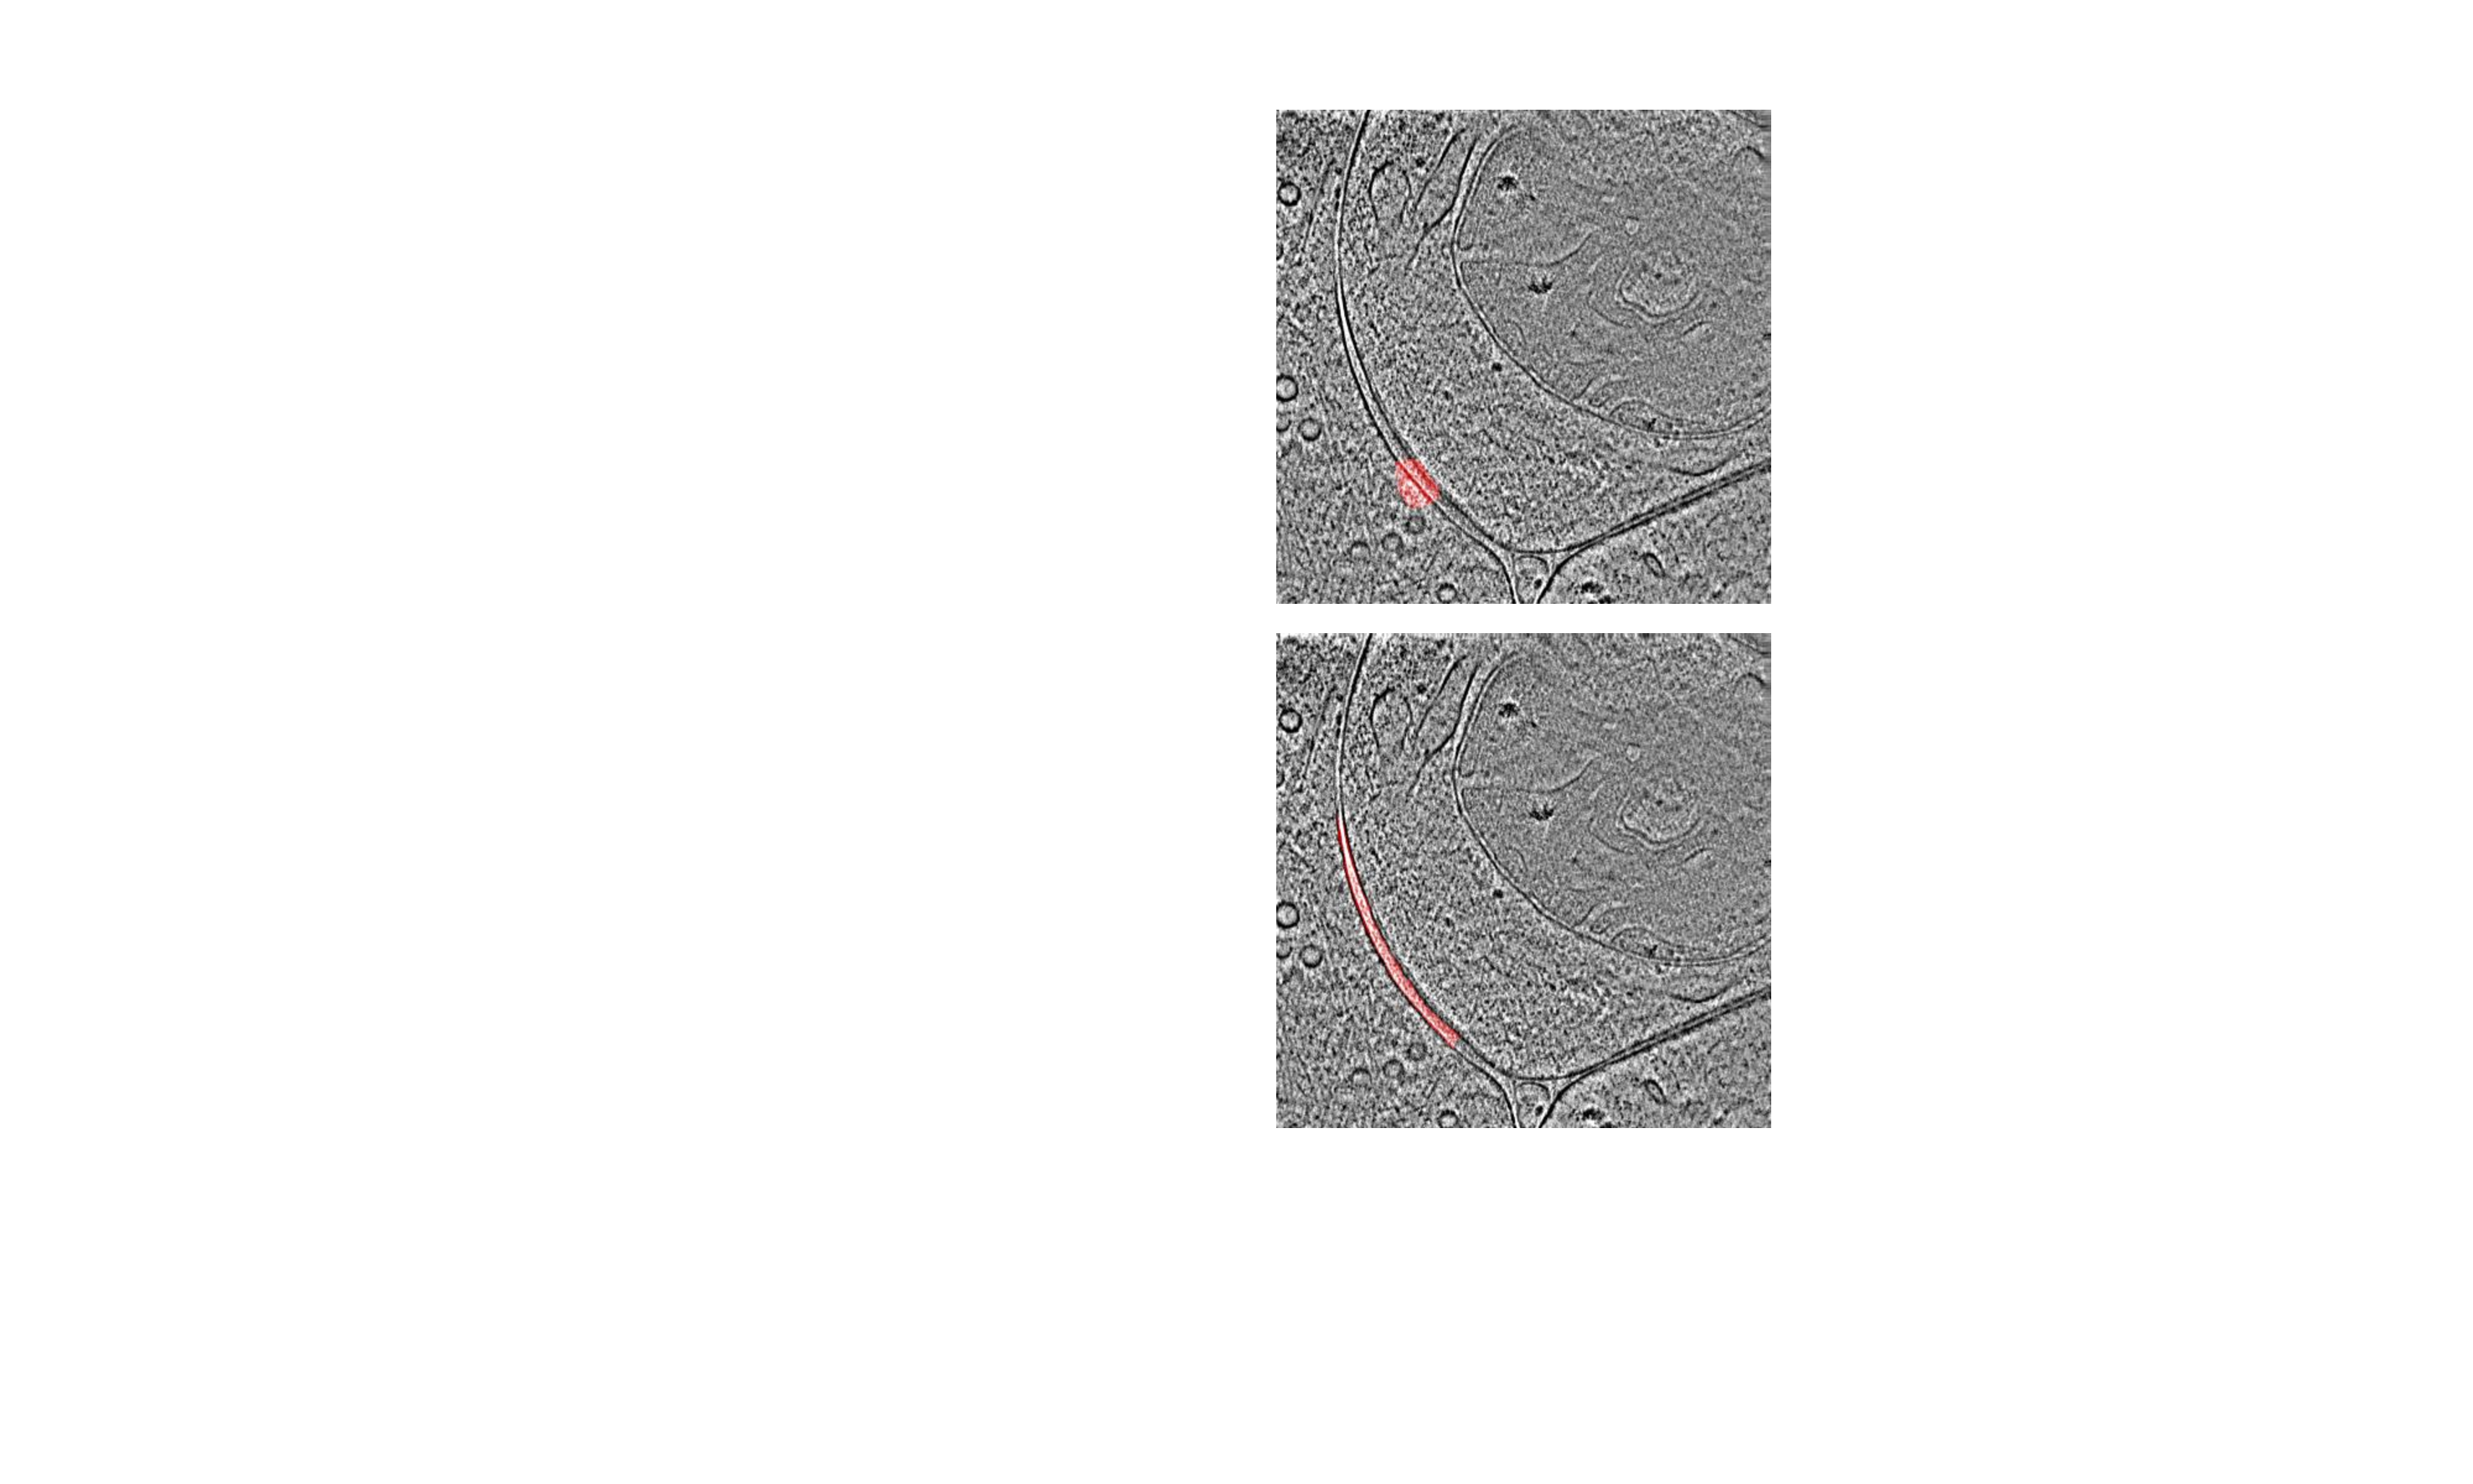
\includegraphics[height=1.6in,width=0.23\columnwidth]{figs/FigSeg2c.pdf}}
    %\hspace{0.05cm}
	\subfigure[PSPNet~\cite{Zhao2016}]{
		\label{fig:seg2:pspnet} %% label for second subfigure
		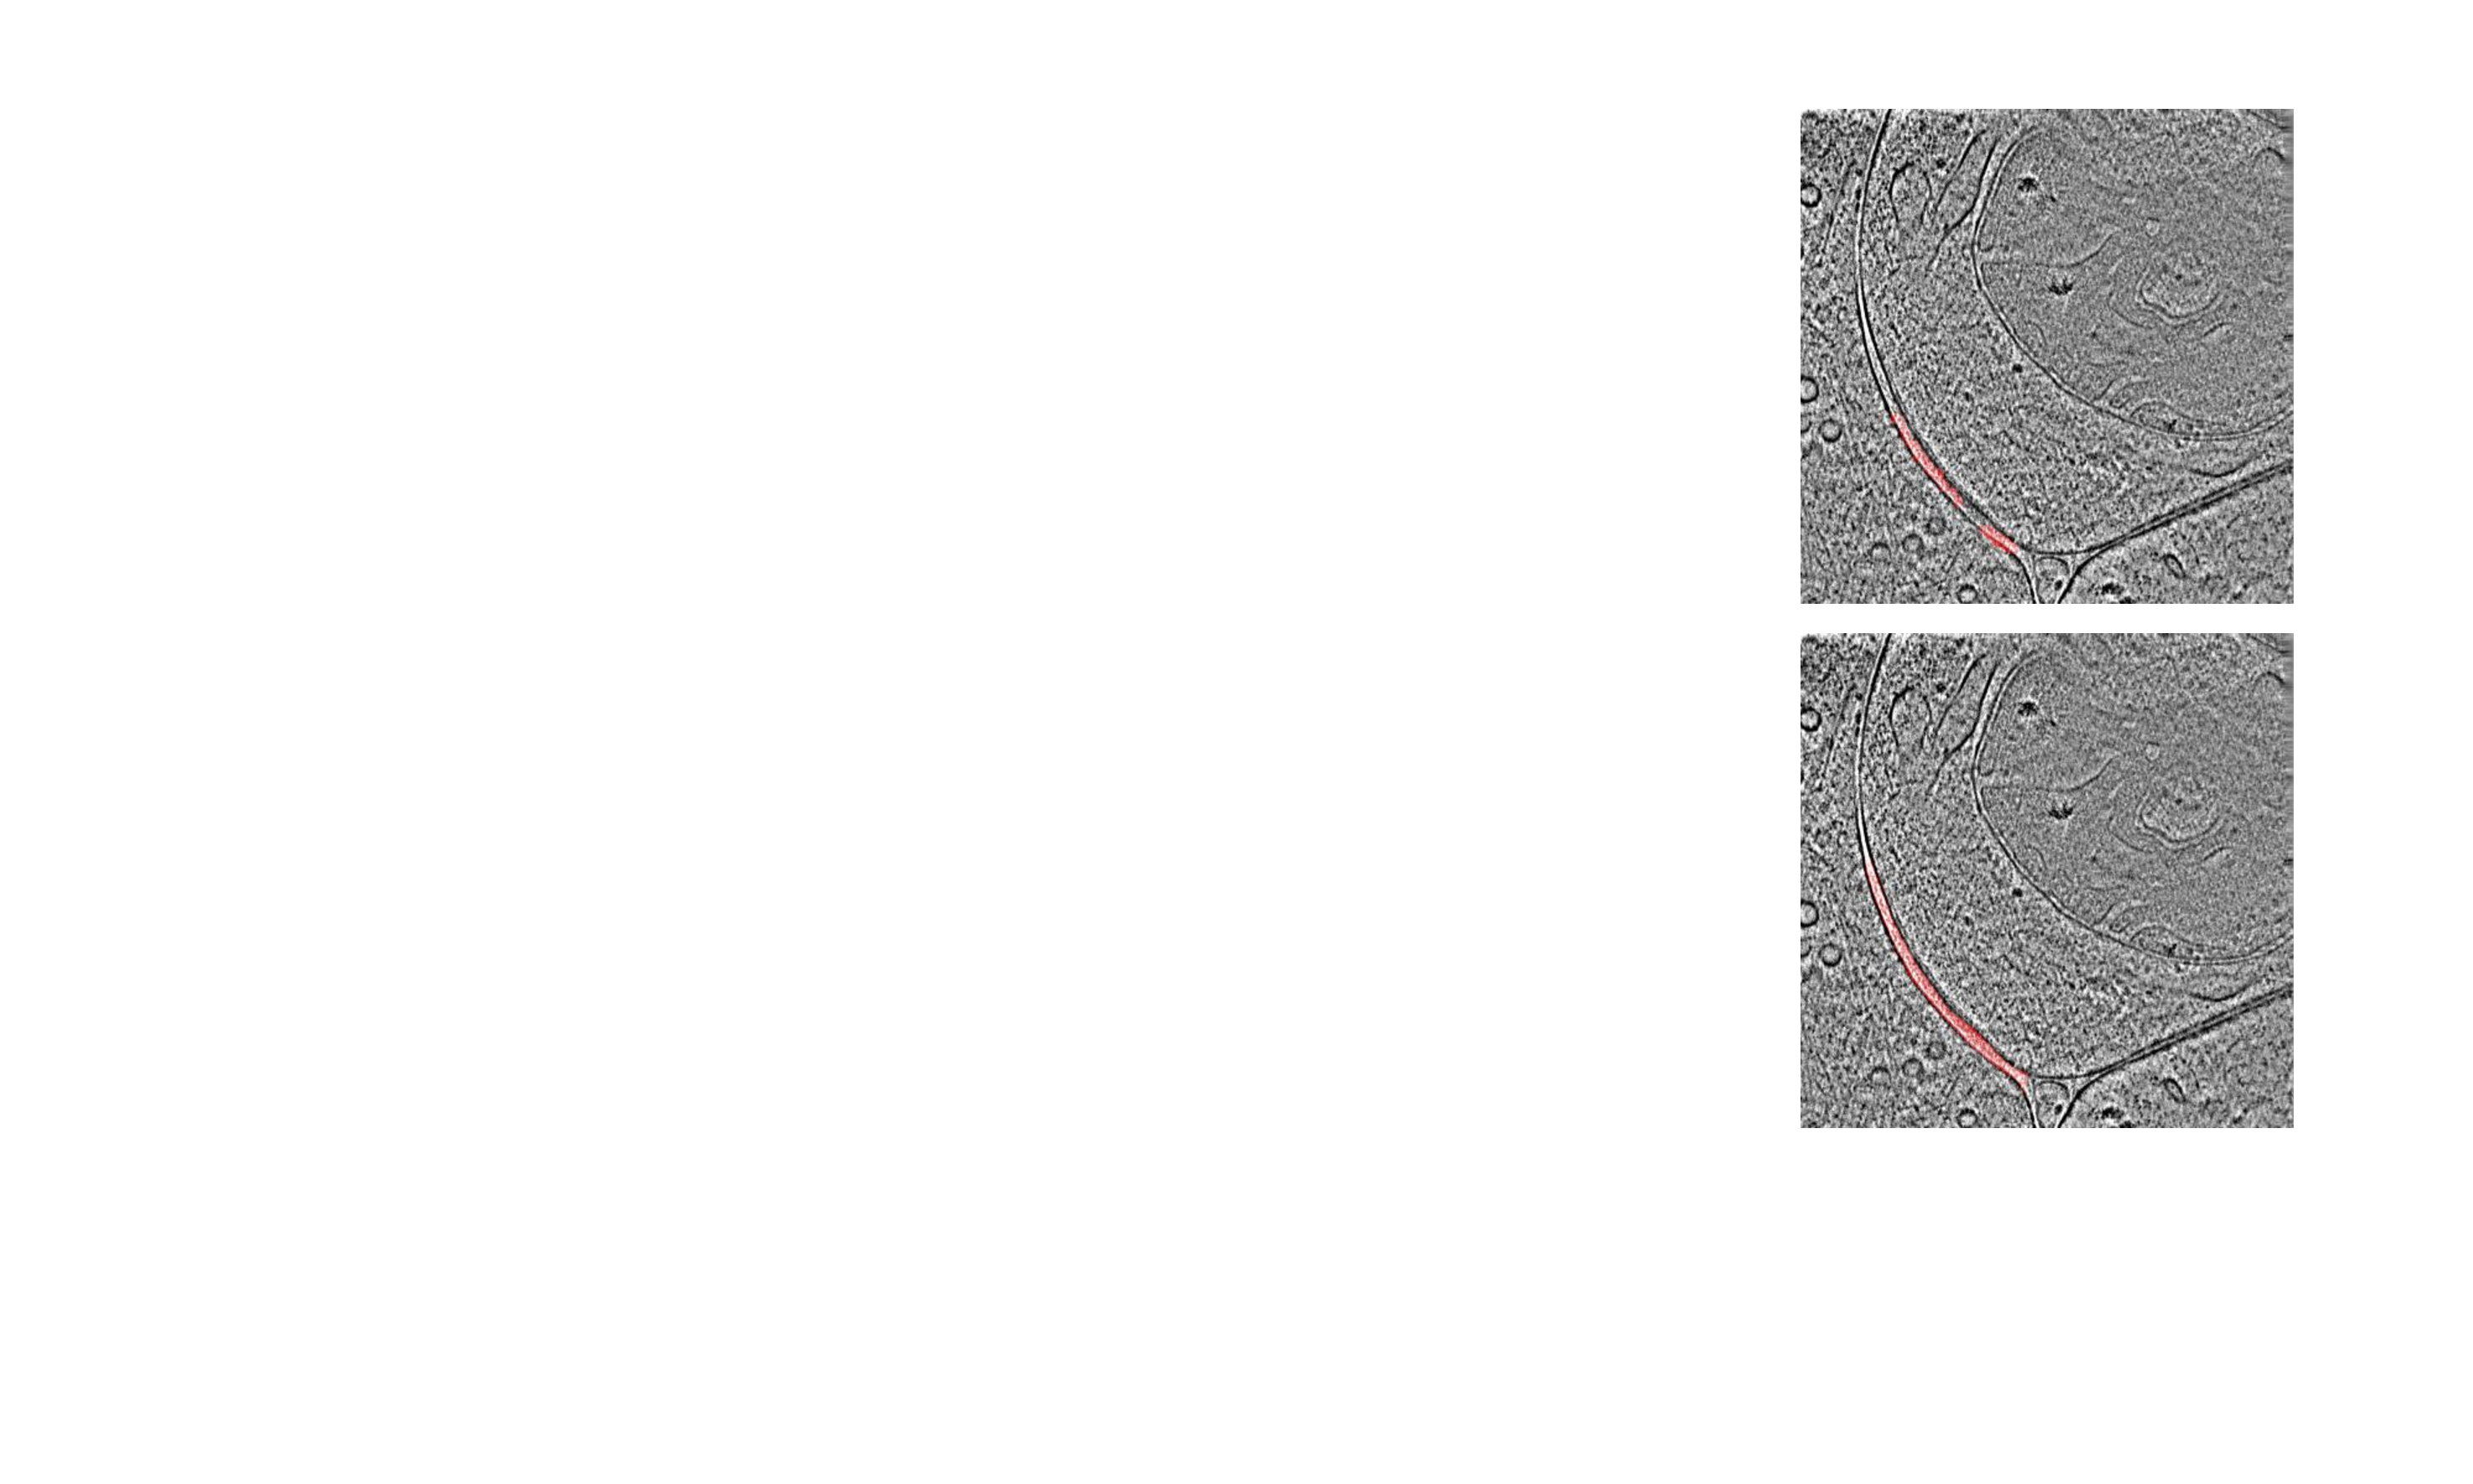
\includegraphics[height=1.6in,width=0.23\columnwidth]{figs/FigSeg2d.pdf}}
	\caption{ Segmentation of our contour growing with different pre-segmentation model.}
	\label{FigSeg2}
\end{figure}